% Tell RStudio that weaving is to be done with the knitr package
% !Rnw weave = knitr


%\listfiles                   %% Show all files used in the book
\documentclass[10pt,krantz2]{krantz}\usepackage[]{graphicx}\usepackage[]{color}
%% maxwidth is the original width if it is less than linewidth
%% otherwise use linewidth (to make sure the graphics do not exceed the margin)
\makeatletter
\def\maxwidth{ %
  \ifdim\Gin@nat@width>\linewidth
    \linewidth
  \else
    \Gin@nat@width
  \fi
}
\makeatother

\definecolor{fgcolor}{rgb}{0.345, 0.345, 0.345}
\newcommand{\hlnum}[1]{\textcolor[rgb]{0.686,0.059,0.569}{#1}}%
\newcommand{\hlstr}[1]{\textcolor[rgb]{0.192,0.494,0.8}{#1}}%
\newcommand{\hlcom}[1]{\textcolor[rgb]{0.678,0.584,0.686}{\textit{#1}}}%
\newcommand{\hlopt}[1]{\textcolor[rgb]{0,0,0}{#1}}%
\newcommand{\hlstd}[1]{\textcolor[rgb]{0.345,0.345,0.345}{#1}}%
\newcommand{\hlkwa}[1]{\textcolor[rgb]{0.161,0.373,0.58}{\textbf{#1}}}%
\newcommand{\hlkwb}[1]{\textcolor[rgb]{0.69,0.353,0.396}{#1}}%
\newcommand{\hlkwc}[1]{\textcolor[rgb]{0.333,0.667,0.333}{#1}}%
\newcommand{\hlkwd}[1]{\textcolor[rgb]{0.737,0.353,0.396}{\textbf{#1}}}%

\usepackage{framed}
\makeatletter
\newenvironment{kframe}{%
 \def\at@end@of@kframe{}%
 \ifinner\ifhmode%
  \def\at@end@of@kframe{\end{minipage}}%
  \begin{minipage}{\columnwidth}%
 \fi\fi%
 \def\FrameCommand##1{\hskip\@totalleftmargin \hskip-\fboxsep
 \colorbox{shadecolor}{##1}\hskip-\fboxsep
     % There is no \\@totalrightmargin, so:
     \hskip-\linewidth \hskip-\@totalleftmargin \hskip\columnwidth}%
 \MakeFramed {\advance\hsize-\width
   \@totalleftmargin\z@ \linewidth\hsize
   \@setminipage}}%
 {\par\unskip\endMakeFramed%
 \at@end@of@kframe}
\makeatother

\definecolor{shadecolor}{rgb}{.97, .97, .97}
\definecolor{messagecolor}{rgb}{0, 0, 0}
\definecolor{warningcolor}{rgb}{1, 0, 1}
\definecolor{errorcolor}{rgb}{1, 0, 0}
\newenvironment{knitrout}{}{} % an empty environment to be redefined in TeX

\usepackage{alltt}
%\documentclass[11pt]{book}
%\usepackage{amsmath}
\usepackage{array}            %% nicer arrays and tables
\usepackage{times}            %% PS Times, rather than CM fonts
\usepackage[T1]{fontenc}      %% for non-alpha chars in \tt
\usepackage{sfheaders}        %% Chap/Sec headers in Helvetica
\usepackage{graphicx}         %% well, its about graphics
\usepackage{alltt}            %% for source listings
\usepackage{mdwlist}          %% Compressed list environments: itemize*, description*, etc.
\usepackage{comment}          %% Stuff commented out
\usepackage{xspace}           %% Smart spacing after tex macros
\usepackage[obeyspaces]{url}  %% URLs and pathnames
\usepackage{bm}               %% for bold math symbols (via \vec{}, \mat{})
\usepackage[tc]{titlepic}     %% Used for the cover illustration
\usepackage{showlabels}       %% Used for checking xrefs
\renewcommand{\showlabelfont}{\footnotesize\ttfamily}
\usepackage{tikz}             %% used for hyp3way.tex
% colored tables
\usepackage{xcolor,colortbl}  %% used ub Ch 01
\usepackage{multirow}
%\usepackage[traceon]{changebar}  %% When we need to show diffs
\usepackage{epigraph}         %% section quotations
\setlength{\epigraphwidth}{.8\textwidth}
%% indexing
\usepackage{index}          

\usepackage[comma]{natbib}
\renewcommand{\bibname}{References}
%\bibliographystyle{abbrvnat-apa}  % this includes URLs
\bibliographystyle{abbrvnat-apa-nourl}

%%%%%%%%%%%%%%%%%%%%%%%%%%%%%%%%%%%%%%%%%%%%%%%%%
%% Setup page style mods from krantz style
%%%%%%%%%%%%%%%%%%%%%%%%%%%%%%%%%%%%%%%%%%%%%%%%%
%

% figure/table names
\renewcommand\figurename{Figure}
\renewcommand\tablename{Table}

% override default to use chapter/section headers
\makeatletter
\def\HeadingsChapterSection{%
  \def\chaptermark##1{%
    \markboth{%
      \thechapter. ##1}{}}%
  \def\sectionmark##1{%
    \markright{%
      \thesection: ##1}}}
\HeadingsChapterSection

\def\@TableTitle{%
  \noindent
  {%
    \vbox{{\TableNumberFont Table\ \thetable}}\par\TableTitleFont\@tabletitle}}

\long\def\@makecaption#1#2{%
  \vskip\abovecaptionskip
  \sbox\@tempboxa{#1: #2}%
  \ifdim \wd\@tempboxa >\hsize
    {\FigCapFont #1:} #2\par
  \else
    \global \@minipagefalse
%    \hb@xt@\hsize{\hfil\box\@tempboxa\hfil}%
    {\FigCapFont #1:} #2\par
  \fi
  \vskip\belowcaptionskip}
\makeatother


% %% Page Headings
% %\makeatletter
% \usepackage{fancyhdr}
% \pagestyle{fancy}
% % \addtolength{\headwidth}{\marginparsep}
% % \addtolength{\headwidth}{\marginparwidth}
% % \addtolength{\headheight}{1.6pt}   %% suppress overfull \vbox chatter
% %
% %% The next two lines are only for draft printing
% %\def\infoleft{\quad [{\small\ttfamily\@filef@und}]}
% % \def\infoleft{[\number\month-\number\day-\number\year]\quad}
% % \def\inforight{[\number\month-\number\day-\number\year]\quad}
% %
% \renewcommand{\chaptermark}[1]{%
%  \markboth{\thechapter\ #1}{}}
% \renewcommand{\sectionmark}[1]{%
%  \markright{\thesection\ #1}}
% % \lhead[\fancyplain{}{\bfseries\sffamily\thepage}]%
% %       {\fancyplain{}{{\bfseries\sffamily\rightmark}\infoleft}}
% % \rhead[\fancyplain{}{\inforight{\bfseries\sffamily\leftmark}}]%
% %       {\fancyplain{}{\bfseries\sffamily\thepage}}
% % \cfoot{}
% %\makeatother

%%%%%%%%%%%%%%%%%%%%%%%%%%%%%%%%%%%%%%%%%%%%%%%%
%% Indexing -- only main index for now
%%%%%%%%%%%%%%%%%%%%%%%%%%%%%%%%%%%%%%%%%%%%%%%%

%\makeglossary
\usepackage{index}
\makeindex
\newindex{xmp}{ide}{ine}{Example Index}

% %% Page Headings
% \makeatletter
% \usepackage{fancyhdr}
% \pagestyle{fancy}
% \addtolength{\headwidth}{\marginparsep}
% \addtolength{\headwidth}{\marginparwidth}
% \addtolength{\headheight}{1.6pt}   %% suppress overfull \vbox chatter
% %
% %% The next two lines are only for draft printing
% \def\infoleft{\quad [{\small\ttfamily\@filef@und}]}
% \def\inforight{[\number\month-\number\day-\number\year]\quad}
% %
% \renewcommand{\chaptermark}[1]{%
%  \markboth{\thechapter\ #1}{}}
% \renewcommand{\sectionmark}[1]{%
%  \markright{\thesection\ #1}}
% \lhead[\fancyplain{}{\bfseries\sffamily\thepage}]%
%       {\fancyplain{}{{\bfseries\sffamily\rightmark}\infoleft}}
% \rhead[\fancyplain{}{\inforight{\bfseries\sffamily\leftmark}}]%
%       {\fancyplain{}{\bfseries\sffamily\thepage}}
% \cfoot{}
% \makeatother

%%%%%%%%%%%%%%%%%%%%%%%%%%%%%%%%%%%%%%%%%%%%%%%%
% Only for chapter.Rnw
\usepackage{xr}
\externaldocument{book}
%%%%%%%%%%%%%%%%%%%%%%%%%%%%%%%%%%%%%%%%%%%%%%%%


% %  Page dimensions
% \addtolength{\hoffset}{-1.1cm}
% \addtolength{\textwidth}{2.2cm}
% \addtolength{\voffset}{-2cm}
% \addtolength{\textheight}{4cm}
% \setlength{\parskip}{3pt plus 1pt}
% \addtolength\marginparwidth {-.5cm}
% 
% % Float parameters
% \renewcommand\textfraction{.15}
% \renewcommand\topfraction{.8}
% % the rest are the defaults
% \setcounter{topnumber}{2}
% \setcounter{bottomnumber}{1}
% \renewcommand\bottomfraction{.3}
% \setcounter{totalnumber}{3}
% \renewcommand\floatpagefraction{.5}

% General LaTeX commands for VCDR

%  Math commands
\newcommand{\bvec}[1]{\ensuremath{\mathbf{#1}}}
\renewcommand{\vec}[1]{\ensuremath{\bm{#1}}}
%\newcommand{\mat}[1]{\ensuremath{\mathbf{#1}}}
\newcommand{\mat}[1]{\ensuremath{\bm{#1}}}               % matrix (bold)
\newcommand{\trans}{\ensuremath{^\mathsf{T}}}            % transpose
\newcommand*{\degree}[1]{\ensuremath{{#1}^{\circ}}}
\newcommand{\diag}[1]{\ensuremath{\mathrm{diag}\, #1}}
\def\binom#1#2{{#1 \choose #2}}%
\newcommand*{\comma}{\:\: ,}%                      punct after displaymath
\newcommand*{\period}{\:\: .}
\newcommand*{\given}{\ensuremath{\, | \,}}
\newcommand*{\implies}{\ensuremath{\Longrightarrow}}

\newcommand*{\rank}[1]{\ensuremath{\mathrm{rank} (\mat{#1})}}
\newcommand*{\dev}[1]{(#1 - \bar{#1})}
\newcommand*{\inv}[1]{\ensuremath{\mat{#1}^{-1}}}
\newcommand*{\half}[1]{\ensuremath{\mat{#1}^{1/2}}}
\newcommand*{\nvec}[2]{\ensuremath{{#1}_{1}, {#1}_{2},\ldots,{#1}_{#2}}}
\newcommand*{\E}{\mathcal{E}}
\newcommand*{\V}{\mathcal{V}}
\newcommand{\iid}{\stackrel{iid}{\sim}}

\newcommand{\blacksquare}{\rule{1.4ex}{1.4ex}}

% Coefficient with error underneath
\newcommand{\cwe}[2]{% 
  \mathord{\mathop{#1}\limits_{(#2)}}%
}
\newcommand{\sizedmat}[2]{%
  \mathord{\mathop{\mat{#1}}\limits_{(#2)}}%
}

%%%%%%%%%%%%%%%%%%%%%%%%%%%%%%%%%%%%%%%%%%%%%%%%%%%%%%
% mathematical functions
%%%%%%%%%%%%%%%%%%%%%%%%%%%%%%%%%%%%%%%%%%%%%%%%%%%%%%

\makeatletter
\def\logit{\mathop{\operator@font logit}}
\def\Bin{\mathop{\operator@font Bin}}
\def\Pois{\mathop{\operator@font Pois}}
\def\NBin{\mathop{\operator@font NBin}}
\def\Geom{\mathop{\operator@font Geom}}
\def\sign{\mathop{\operator@font sign}}
\def\Vec{\mathop{\operator@font vec}}

%\newcommand{\min}{\operatornamewithlimits{min}}
%\newcommand{\max}{\operatornamewithlimits{max}}
%\newcommand{\argmin}{\operatornamewithlimits{arg\,min}}
%\newcommand{\argmax}{\operatornamewithlimits{arg\,max}}
% the *ed form allows limits above/below, the non*ed form prints these beside the operator
%\DeclareMathOperator*{\argmin}{arg\,min}

%\newcommand{\Xvec}{X_1,X_2, \ldots, X_n }
% should add an argument for n
\newcommand{\sumi}[2]{\sum_{#1=1}^#2}

\def\ignorespacesafterend{\global\@ignoretrue}
\newenvironment{equation*}
	{\begin{displaymath}}%
%	{\end{displaymath}}%
	{\end{displaymath}\ignorespacesafterend}%
%
% Donald Arseneau recommends:
%\newenvironment{equation*}{\displaymath}{\enddisplaymath}%

%%%%%%%%%%%%%%%%%%%%%%%%%%%%%%%%%%%%%%%%%%%%%%%%%%%%%%
%% common abbreviations
%%%%%%%%%%%%%%%%%%%%%%%%%%%%%%%%%%%%%%%%%%%%%%%%%%%%%%

\newcommand*{\hires}{high-resolution}
\newcommand*{\etal}{\emph{et al.}}
\newcommand*{\loglin}{loglinear\xspace}
\newcommand*{\Loglin}{Loglinear\xspace}
\newcommand*{\ctab}{contingency table\xspace}
\newcommand*{\ctabs}{contingency tables\xspace}
\newcommand*{\mway}{multiway\xspace}
\newcommand*{\LR}{likelihood-ratio\xspace}
\newcommand*{\CA}{Correspondence analysis\xspace}
\newcommand*{\ca}{correspondence analysis\xspace}
\newcommand*{\nway}{\emph{n}-way\xspace}
\newcommand*{\GSQ}{\ensuremath{G^2}\xspace}
\newcommand*{\chisq}{\ensuremath{\chi^2}\xspace}
\newcommand*{\scat}{scatterplot\xspace}
\newcommand*{\scats}{scatterplots\xspace}
\newcommand*{\scatmat}{\scat{} matrix\xspace}
\newcommand*{\df}{degrees of freedom\xspace}
\newcommand*{\Dset}{data set\xspace}
\newcommand*{\Dsets}{data set\xspace}

%% notation for loglinear models [AB][C] -- now use \mathrm{}
\newcommand*{\llmterm}[1]{\ensuremath{[}#1\ensuremath{]}}
%\newcommand*{\llmterm}[1]{\ensuremath{[}\ensuremath{\mathrm{#1}\ensuremath{]}}
%\newcommand*{\llmterm}[1]{\ensuremath{[\mathrm{#1}]}
\newcommand*{\llmtwo}[2]{\llmterm{#1} \llmterm{#2}}
\newcommand*{\llmthree}[3]{\llmterm{#1} \llmterm{#2} \llmterm{#3}}
\newcommand*{\llmfour}[4]{\llmterm{#1} \llmterm{#2} \llmterm{#3} \llmterm{#4}}

%% \LLM{A,B,C} --> [A] [B] [C] for loglin models
\DeclareRobustCommand*{\LLM}[1]{%
%\def\LLM#1{%
	\@for\@term:=#1\do{%
	\llmterm{\@term}%
	}
}
\makeatother

% deprecated, but maybe used somewhere
\newcommand*{\boldital}[1]{\textit{\textbf{#1}}}

%%%%%%%%%%%%%%%%%%%%%%%%%%%%%%%%%%%%%%%%%%%%%%%%%%%%%%%%%%%%%%%%%%
% precept -- something to stand out in the text
%   could use a box or something else
%%%%%%%%%%%%%%%%%%%%%%%%%%%%%%%%%%%%%%%%%%%%%%%%%%%%%%%%%%%%%%%%%%

\newcommand{\precept}[1]{%
\begin{quote}
\centering
\textbf{#1}
\end{quote}
}


%%%%%%%%%%%%%%%%%%%%%%%%%%%%%%%%%%%%%%%%%%%%%%%%%%%%%%%%%%%%%%%%%%
% \glossterm -- used for terms that should be highlighted in the
% text and index, and which might go into a glossary (but only 
% if glosstex is run)
% The original definition did not allow for such terms at the beginning
% of a sentence.
%\newcommand{\glossterm}[1]{\textit{\textbf{#1}}\glosstex{#1}}

% Simple variant, just for formatting; can also use \marginpar{}
% and glossterm
\newcommand{\term}[1]{\textit{\textbf{#1}}\index{#1}}

%\glossterm[print-form]{gloss-form}
\makeatletter
\def\glossterm{\@dblarg\@glossterm}
\def\@glossterm[#1]#2{\textit{\textbf{#1}}\glosstex{#2}\index{#2|textbf}}
\makeatother

% Author's notes -- to disappear in production
\newcommand{\aunote}[1]{\marginpar{\footnotesize\textbf{Au:} #1}}

% Dummy command for changes
%\newenvironment{changebar}{}{}%
%\newcommand{\changebar}[1]{#1}

%%%%%%%%%%%%%%%%%%%%%%%%%%%%%%%%%%%%%%%%%%%%%%%%%%%%%%%%%%%%%%%%%%%%%%
% Commands to simplify cross-references
%%%%%%%%%%%%%%%%%%%%%%%%%%%%%%%%%%%%%%%%%%%%%%%%%%%%%%%%%%%%%%%%%%%%%%

\newcommand*{\eqref}[1]{Eqn.~(\ref{#1})}
\newcommand*{\exref}[1]{Example~\ref{#1}}
\newcommand*{\chref}[1]{Chapter~\ref{#1}}
\newcommand*{\secref}[1]{Section~\ref{#1}}
\newcommand*{\figref}[1]{Figure~\ref{#1}}
\newcommand*{\tabref}[1]{Table~\ref{#1}}
\newcommand*{\outref}[1]{Output~\ref{#1}}
\newcommand*{\datref}[1]{Appendix~\ref{#1}}
%\newcommand*{\macref}[1]{Appendix~\ref{#1}}
\newcommand*{\appref}[1]{Appendix~\ref{#1}}

% Reference a range of refs
\newcommand*{\chrange}[2]{Chapters~\ref{#1}--\ref{#2}}
\newcommand*{\figrange}[2]{Figures~\ref{#1}--\ref{#2}}
\newcommand*{\tabrange}[2]{Tables~\ref{#1}--\ref{#2}}
%
% Reference a list of figs, examples, etc., not necessarily sequential
\newcommand{\figrefs}[1]{\dorefs{#1}{Figures}}
\newcommand{\tabrefs}[1]{\dorefs{#1}{Tables}}
\newcommand{\exrefs}[1]{\dorefs{#1}{Examples}}
\makeatletter
\newcommand{\dorefs}[2]{%
  \let\@dummy\@empty
  #2~%
  \@for\@term:=#1\do{%
    \@dummy
    \edef\@dummy{\ref{\@term}, }}%
  \expandafter\format@last\@dummy}
\def\format@last#1, {and #1}
\makeatother


%%%%%%%%%%%%%%%%%%%%%%%%%%%%%%%%%%%%%%%%%%%%%%%%%%%%%%%%%%%%%%%%%%%%%%%%%%%
% multiline headers in tables 
% use as: Variable & DF & \multilineC{Parameter \\ Estimate} & ...
%%%%%%%%%%%%%%%%%%%%%%%%%%%%%%%%%%%%%%%%%%%%%%%%%%%%%%%%%%%%%%%%%%%%%%%%%%%

\newcommand{\multilineR}[1]{\begin{tabular}[b]{@{}r@{}}#1\end{tabular}} 
\newcommand{\multilineL}[1]{\begin{tabular}[b]{@{}l@{}}#1\end{tabular}} 
\newcommand{\multilineC}[1]{\begin{tabular}[b]{@{}c@{}}#1\end{tabular}} 

%% table stuff, another way
% to make it easier to use & \brk{this\\or\\that} & in \tabular

\newcommand{\brk}[2][l]{%
   \begin{tabular}{@{}#1@{}}#2%
   \end{tabular}%
}

%%%%%%%%%%%%%%%%%%%%%%%%%%%%%%%%%%%%%%%%%%%%%%%%%%%%%%%%%%%%%%%%%%%%%%%%%%%%
% colored tables
%%%%%%%%%%%%%%%%%%%%%%%%%%%%%%%%%%%%%%%%%%%%%%%%%%%%%%%%%%%%%%%%%%%%%%%%%%%%
% requires:
%\usepackage{xcolor,colortbl}  %% used ub Ch 01

%\newcommand{\tableheader}{\rowcolor[gray]{.85}}
\newcommand{\tableheader}{\rowcolor[HTML]{FFFFC7}} % light yellow background

\newcommand{\cell}[2]{\multicolumn{1}%
   {>{\columncolor{#1}}r}{#2}}

\newcommand{\C}{Chapter\xspace}

\newcommand{\chapterprelude}[1]{%
\textsf{#1}
\newline
\rule{\textwidth}{0.4pt}
}


%\renewcommand{\S}{Section }

%%%%%%%%%%%%%%%%%%%%%%%%%%%%%%%%%%%%%%%%%%%%%%%%%%%%%%%%%%%%%%%
% R terminology

% writing about R stuff; these can be modified to add indexing, etc.
\newcommand{\var}[1]{\texttt{#1}}

% Data sets -- print and index
%\newcommand{\data}[1]{\texttt{#1}}
\newcommand*{\data}[1]{\textit{\texttt{#1}}\ixd{#1}}

\newcommand{\class}[1]{\textsf{"#1"}}

% may need a more robust version of \code to handle special chars
% this doesn't quite handle it.
% Added \sloppy to avoid \hbox too wide problems
\makeatletter
\newcommand\code{\bgroup\@makeother\_\@makeother\~\@makeother\$\@codex}
\def\@codex#1{{\sloppy\normalfont\ttfamily\hyphenchar\font=-1 #1}\egroup}
\makeatother
%\newcommand{\code}[1]{\texttt{#1}}

% R functions: use \code{} and also \index{}
\newcommand{\func}[1]{\code{#1()}\ixfunc{#1}}

\let\proglang=\textsf
\newcommand{\R}{\proglang{R}\xspace}

% should redefine \pkg to also cite the package, but this requires
% an extra, optional argument, unless it is assured that the package
% name is the bibtex key; also: add indexing
%\newcommand{\pkg}[1]{{\normalfont\fontseries{b}\selectfont #1}}
%\newcommand{\pkg}[1]{\textsf{#1}\ixp{#1}}

% reference and \cite a package, but only on first use
\def\pkg#1{\textsf{#1}\ixp{#1}~\citex{#1}\xspace}
\def\citex#1{\expandafter\ifx\csname cit:#1\endcsname\relax
      \expandafter\gdef\csname cit:#1\endcsname{}%
      \citep{#1}%
   \else
      \nocite{#1}%
   \fi
}

\newcommand{\Rpackage}[1]{\pkg{#1} package}

% R base packages all have the same reference -- shouldn't be cited
\newcommand{\basepkg}[1]{\textsf{#1}\ixp{#1}}



\newcommand{\help}[1]{\code{help(#1)}}     % reference R help

\newcommand*{\VCDR}{\emph{VCDR} }
\newcommand*{\argument}[1]{\texttt{#1} argument}
%\newcommand*{\sasprog}[1]{\texttt{#1} program\ixp{#1}}
%\newcommand*{\default}[1]{\texttt{[}Default: \url{#1}\texttt{]}}

%%%%%%%%%%%%%%%%%%%%%%%%%%%%%%%%%%%%%%%%%%%%%%%%%%%%%%%%%%%%%%%%%%%%%%%
% Index generation
% Indexentry for a word/phrase (Word inserted into the text)
%%%%%%%%%%%%%%%%%%%%%%%%%%%%%%%%%%%%%%%%%%%%%%%%%%%%%%%%%%%%%%%%%%%%%%%
\newcommand{\IX}[1]{\index{#1}#1}
\newcommand{\ix}[1]{\index{#1}}
\newcommand{\ixmain}[1]{\index{#1|textbf}}

%\newcommand{\ixm}[1]{%
%   \index{#1@\texttt{#1} macro}%
%   \index{macros!#1@\texttt{#1}}%
%	}

% R functions
\newcommand{\ixfunc}[1]{%
  \index{#1@\texttt{#1()}}%
%  \index{functions!#1@\texttt{#1}}%
 }

% R packages:  indexed under both package name and packages!
\newcommand{\ixp}[1]{%
   \index{#1@\textsf{#1} package}%
   \index{package!#1@\textsf{#1}}%
	}


% data sets: 
\newcommand{\ixd}[1]{%
        \index{data sets!#1}}

% Examples Index
\newcommand{\ixe}[1]{\index[xmp]{#1}}
\newcommand{\ixeon}[1]{\ixe{#1|(}}      % when not automatically done by Example
\newcommand{\ixeoff}[1]{\ixe{#1|)}}

\newcommand{\ixon}[1]{\index{#1|(}}
\newcommand{\ixoff}[1]{\index{#1|)}}


%\newcommand*\seealso[2]{\emph{\alsoname} #1}
% and then:
%\index{foo|seealso{bar}}
% If \alsoname isn't defined, you would have to add:
%\newcommand{\alsoname}{see also}

% This puts the argument in italics in the text, in boldface in the
% index, and if you give an optional argument, that goes in the index,
% so you can write:

%\define{gnat}
%\define[animals|gnats]{gnat}

\makeatletter
\newcommand{\define}{\@ifnextchar[\@dfna\@dfnb}
\def\@dfna[#1]#2{\textit{#2}\index{#1|textbf}}
\def\@dfnb#1{\@dfna[#1]{#1}}
\makeatother

%%%%%%%%%%%%%%%%%%%%%%%%%%%%%%%%%%%%%%%%%%%%%%%%%%%%%%%%%%%%%%%%%%%%%%%%%%%
% Some convenience macros for figures --- not used here
% because knitr seems to do things reasonably well without them.

% Define the current fig directory
\newcommand{\figdir}{ch\thechapter/fig/}
% Redefine the current fig directory
\newcommand{\newfigdir}[1]{\renewcommand{\figdir}{#1/fig/}}

% Command to collect graphics file info - ignored for now, but used
% whereever I abbreviate the graphics file 
% from {chX/fig/figure.eps} to {figure}
\newcommand{\graphicsfile}[2]{\relax}

%% \SASfig{file}{include_opts}{label}{caption}
%  This command is no longer used -- all figures use \includegraphics directly

%\newcommand{\SASfig}[4]{%
%  \centering%
%  \includegraphics[#2]{#1}\graphicsfile{\figdir#1}{}%
%  \caption{#4}\label{fig:#3}%
%  }

%% \fig{file}{include_opts}{shortcaption}[extended caption]
%  label is fig:file
\makeatletter
  \newcommand{\fig}[3]{\@ifnextchar[%]
    {\@extr@fig{#1}{#2}{#3}}%
    {\@norm@fig{#1}{#2}{#3}}%
  }
  \def\@extr@fig#1#2#3[#4]{%
    \begin{figure}[htb]%
    \centering%
    \includegraphics[#2]{\figdir#1}%
    \caption[#3]{#3. #4}\label{fig:#1}%
    \end{figure}%
    }
  \newcommand{\@norm@fig}[3]{%
    \begin{figure}[htb]%
    \centering%
    \includegraphics[#2]{\figdir#1}%
    \caption{#3}\label{fig:#1}%
    \end{figure}%
    }


%%%%%%%%%%%%%%%%%%%%%%%%%%%%%%%%%%%%%%%%%%%%%%%%%%%%%%%%%%%%%%%%%%%%%%%%%%
% Specialized kinds of lists
%%%%%%%%%%%%%%%%%%%%%%%%%%%%%%%%%%%%%%%%%%%%%%%%%%%%%%%%%%%%%%%%%%%%%%%%%%


% APA Seriations: ONE level of seriation only.
%  \begin{seriate} \item ... \end{seriate}
%           within a paragraph or sentence

\newcounter{APAenum}
\def\seriate{\@bsphack\begingroup%
   \setcounter{APAenum}{0}%
   \def\item{\addtocounter{APAenum}{1}(\alph{APAenum})\space}%
   \ignorespaces}
\def\endseriate{\endgroup\@esphack}

\makeatother

% definition lists for programs or arguments, with suitable indenting

\newenvironment{proglist}%
 {\begin{list}{}{%
    \settowidth{\labelwidth}{\texttt{PROGRAMSxx}}
         \setlength{\leftmargin}{\labelwidth}
         \addtolength{\leftmargin}{\labelsep}
         \setlength{\parsep}{0.2ex plus0.2ex minus0.2ex}
         \setlength{\itemsep}{0pt}
         \renewcommand{\makelabel}[1]{\texttt{##1\hfill}}}}
 {\end{list}}


%%%%%%%%%%%%%%%%%%%%%%%%%%%%%%%%%%%%%%%%%%%%%%%%%%%%%%%%%%%%%%%%%%%%%%%
% Numbered examples that can be referenced
%%%%%%%%%%%%%%%%%%%%%%%%%%%%%%%%%%%%%%%%%%%%%%%%%%%%%%%%%%%%%%%%%%%%%%%
%
% \newcounter{example}[chapter]
% \renewcommand{\theexample}{\thechapter.\arabic{example}}
% \newenvironment{Example}[2][\theexample]{%
%   \refstepcounter{example}%
%   \label{ex:#1}%
%   \def\theexamplename{#2}%
%   \begin{trivlist}%
%   \item[%
%   % \hskip-\labelsep % idiosyncrasy that needs learning
%     \textbf{\textsc{Example \theexample}:}] %
% 	\textbf{#2}\par
%   \ixe{#2|(}%
%   }{%
% 	\expandafter\ixe\expandafter{\theexamplename|)}%   magic from Bernd
%   \hfill$\triangle$
% %  The triangle used to mark the end of examples can be replaced by any
% %  other character, ... e.g.,
% %  \hfill\blacksquare
% %	\ding{110}% filled black square (using pifont package)
%   \end{trivlist}%
% }
%%%%%%%%%%%%%%%%%%%%%%%%%%%%%%%%%%%%%%%%%%%%%%%%%%%%%%%%%%%%%%%%%%%%%%%
% Numbered examples that can be referenced and produce index entries
%%%%%%%%%%%%%%%%%%%%%%%%%%%%%%%%%%%%%%%%%%%%%%%%%%%%%%%%%%%%%%%%%%%%%%%
%
\usepackage{xparse}

  \newcounter{example}[chapter]
	\renewcommand{\theexample}{\thechapter.\arabic{example}}
	\NewDocumentEnvironment{Example}{+O{\theexample}+m+o}{%
	  \refstepcounter{example}%
	  \label{ex:#1}%
	  \def\theexamplename{#2}%
	  \begin{trivlist}%
	  \item[%
	  % \hskip-\labelsep % idiosyncrasy that needs learning
	    \textbf{\textsc{Example \theexample}:}] %
	    \IfValueTF{#3}{%
	    \textbf{#2 -- #3}\par
	      \index[xmp]{#2!#3|(}
	    }{%
	    \textbf{#2}\par
	      \index[xmp]{#2|(}
	    }}{%
	    \IfValueTF{#3}{%
	      \index[xmp]{#2!#3|)}
	    }{%
	      \index[xmp]{#2|)}
	    }
	    \hfill$\triangle$
	  \end{trivlist}%
	}

%%%%%%%%%%%%%%%%%%%%%%%%%%%%%%%%%%%%%%%%%%%%%%%%%%%%%%%%%%%%%%%%%%
% Define new list type for exercises
% from: http://tex.stackexchange.com/questions/196199/exercise-list-using-enumitem-how-control-indentation-and-labeling-of-sublists
% by: Daniel Wunderlich
%%%%%%%%%%%%%%%%%%%%%%%%%%%%%%%%%%%%%%%%%%%%%%%%%%%%%%%%%%%%%%%%%%
%
\usepackage{enumitem}      % this should be loaded in book.Rnw
%
\newlist{Exercises}{enumerate}{2}
% set list style parameters
\setlist[Exercises]{%
  label=\textbf{Exercise \thechapter.\arabic*}~,  % Label: Exercise Chapter.exercise
  ref=\thechapter.\arabic*, % References: Chapter.exercise (important!)
  align=left,               % Left align labels
  labelindent=0pt,          % No space betw. margin of list and label
  leftmargin=0pt,           % No space betw. margin of list and following lines
  itemindent=!,             % Indention of item computed automatically
  itemsep=3pt,
}

\newcommand{\exercise}{%
  \item\label{lab:\arabic{chapter}.\arabic{Exercisesi}}%      % Append label to item
  \setlist[enumerate, 1]{label=(\alph*),itemsep=0pt}          % Label for subexercises, but only within an exercise
}

% references to exercises
\newcommand{\labref}[1]{Exercise~\ref{#1}}

%%%%%%%%%%%%%%%%%%%%%%%%%%%%%%%%%%%%%%%%%%%%%%%%%%%%%%%%%%%%%%%%%%%%
%  Author notes, etc

\newcommand{\TODO}[1]{\noindent{\color{red}\textbf{TODO}: #1}}
\newcommand{\DONE}[1]{\noindent{\color{blue}\textbf{Done}: #1}}
% convert these to ignore the supplied text when no longer needed
%\newcommand{\TODO}[1]{\relax}
%\newcommand{\DONE}[1]{\relax}



%% Latex notes, p 73
\newlength{\boxedparwidth}
\setlength{\boxedparwidth}{.92\textwidth}
\newenvironment{boxedtext}%
        {\begin{center}%
         \begin{tabular}{|@{\hspace{.15in}}c@{\hspace{.15in}}|}
         \hline \\ begin{minipage}[t]{\boxedparwidth}
         }
         {\end{minipage} \\ \\ \hline \end{tabular} \end{center}}




%%%%%%%%%%%%%%%%%%%%%%%%%%%%%%%%%%%%%%%%%%%%%%%%%%%%%%%%%%%%%%%%%%%%%%
% Symbols for hard or difficult sections and problems

% -- tried using \dbend, a la TeXbook, but it doesn't look right
% \usepackage{manfnt}
% \newcommand{\hard}{\marginpar{\dbend}}
% \newcommand{\veryhard}{\marginpar{\dbend \dbend}}

\newcommand{\hard}{$^\star$\xspace}
\newcommand{\veryhard}{$^{\star\star}$\xspace}

% need these for exercises
% see http://tex.stackexchange.com/questions/223505/marking-hard-exercises-in-a-book-with-enumitem
\newcommand{\exhard}{\hspace*{-\labelsep}\hard}
\newcommand{\exveryhard}{\hspace*{-\labelsep}\veryhard}


\endinput

\renewenvironment{knitrout}{\small\renewcommand{\baselinestretch}{.85}}{} % an empty environment to be redefined in TeX

%% Shut up some overfull hboxes
\hfuzz=12pt

%%%%  end{preamble}   %%%%%


% % Ch 1
% \setcounter{chapter}{0} % one less than chapter number
% \setcounter{page}{0}    % one less than book page number
% 
% % Ch 2
% \setcounter{chapter}{1} % one less than chapter number
% \setcounter{page}{18}   % one less than book page number
% 
% % Ch 3
% \setcounter{chapter}{2} % one less than chapter number
% \setcounter{page}{50}   % one less than  book page number
% 

%%%%%%%%%%%%%%%%%%%%%%%%%%%%%%%%%%%%%%%%%%%%%%%%%%%%%%%%%%%%%%%%%%%%%%%%%
% Set chapter number in this chunk; edit the page numbers as they change

\setcounter{chapter}{1}\setcounter{page}{26}

\IfFileExists{upquote.sty}{\usepackage{upquote}}{}
\begin{document}







\chapter{Working with categorical data}\label{ch:working}
%\begin{center}
 \rule[-4pt]{0.5pt}{4pt}\hrulefill\rule[-4pt]{0.5pt}{4pt}\\
 \begin{minipage}[c]{.33\linewidth}
  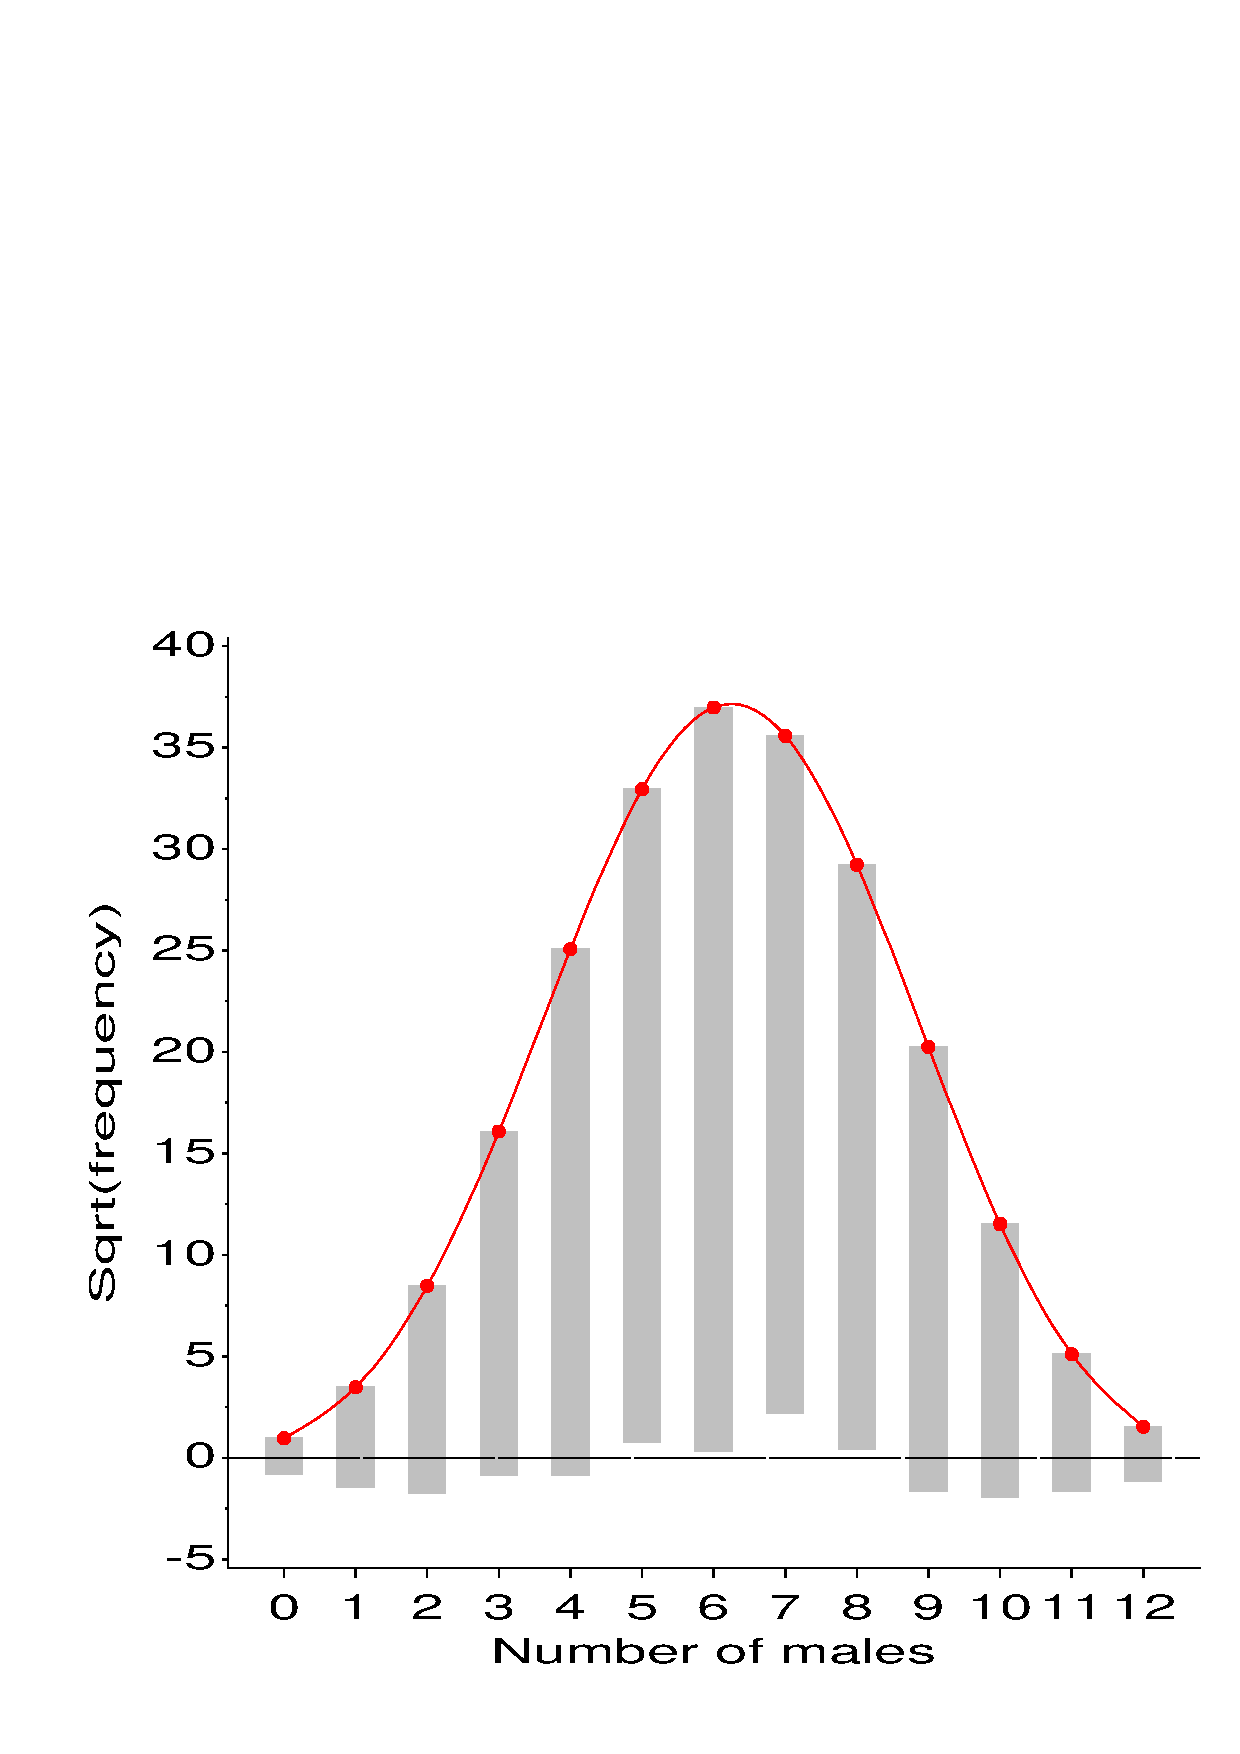
\includegraphics[width=1\linewidth]{saxony}\graphicsfile{ch2/fig/saxony.eps}{}
 \end{minipage}%
 \hfill
 \begin{minipage}[c]{.33\linewidth}
  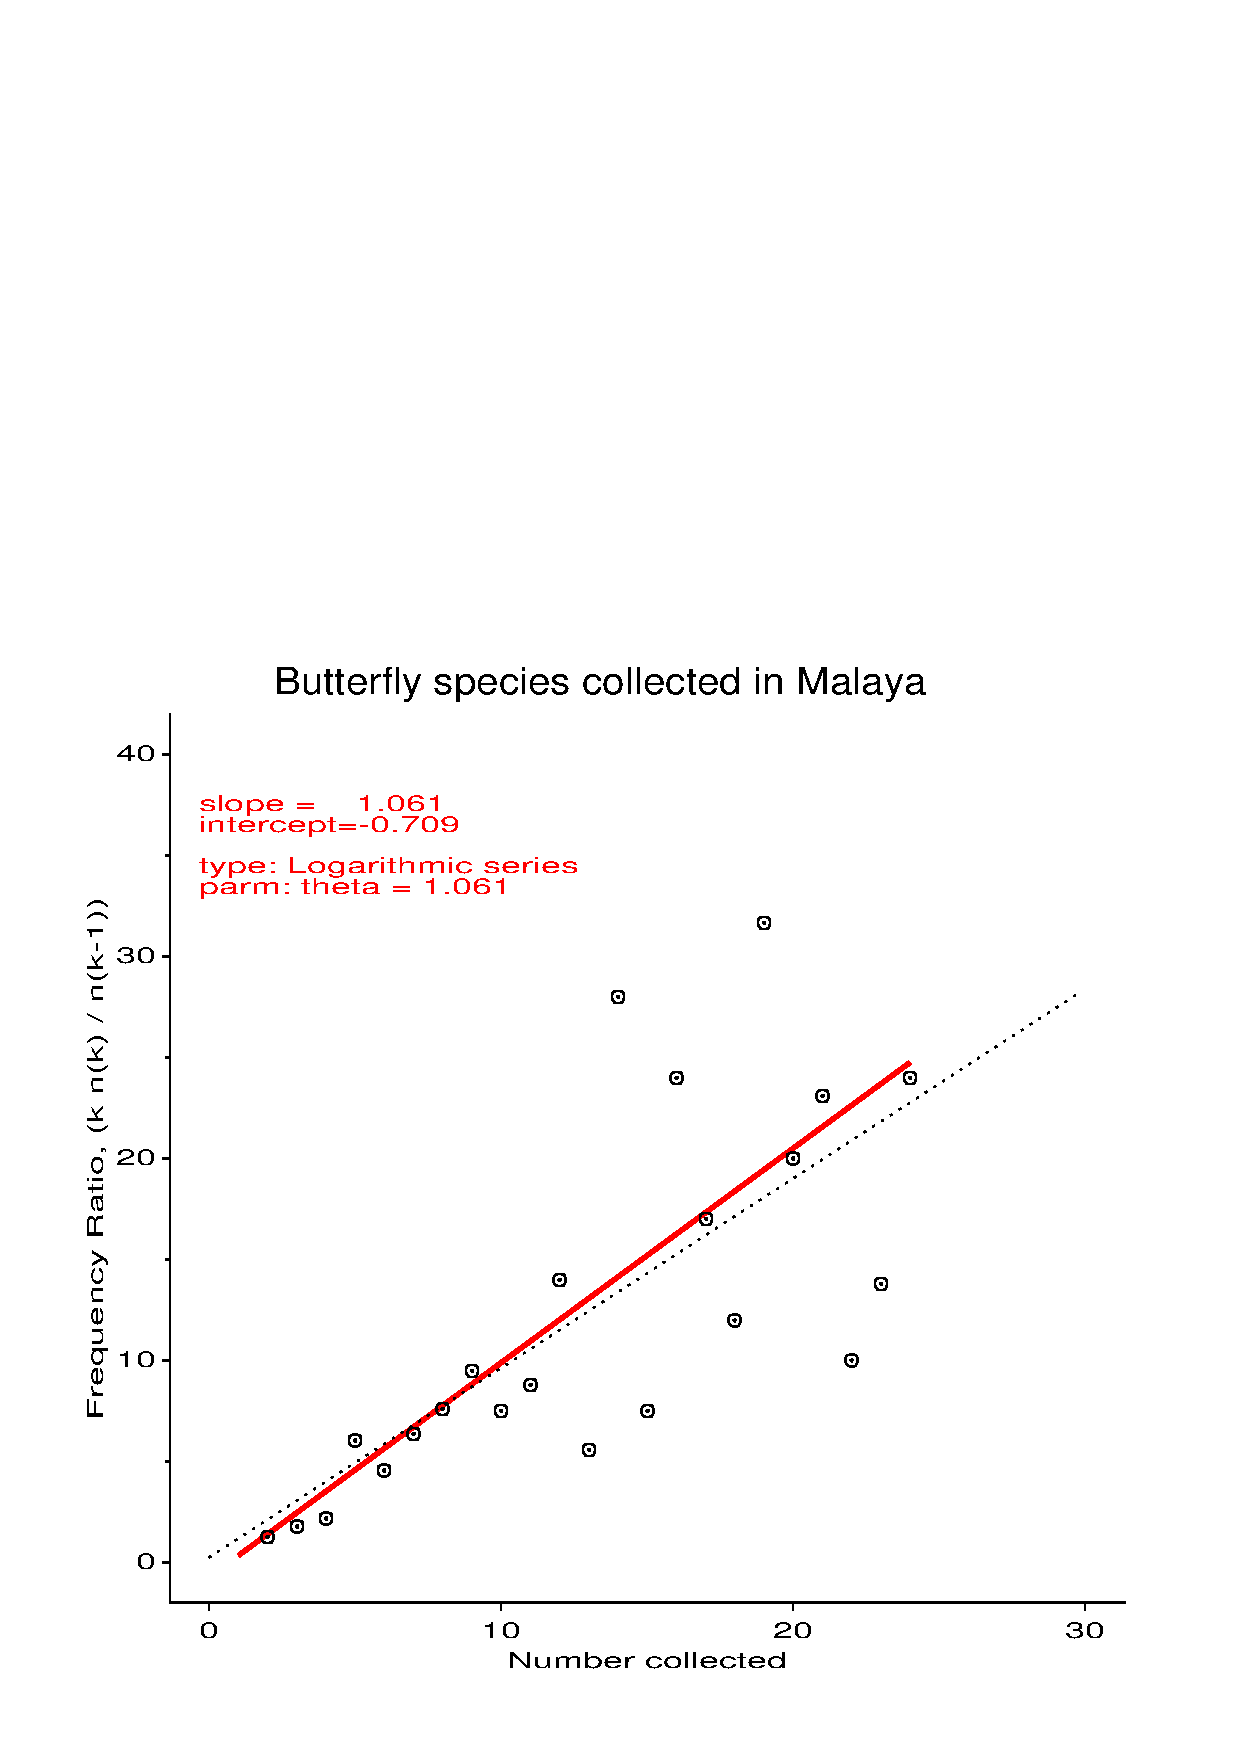
\includegraphics[width=1\linewidth]{orddemo3}\graphicsfile{ch2/fig/orddemo3.eps}{}
 \end{minipage}
 \hfill
 \begin{minipage}[c]{.33\linewidth}
  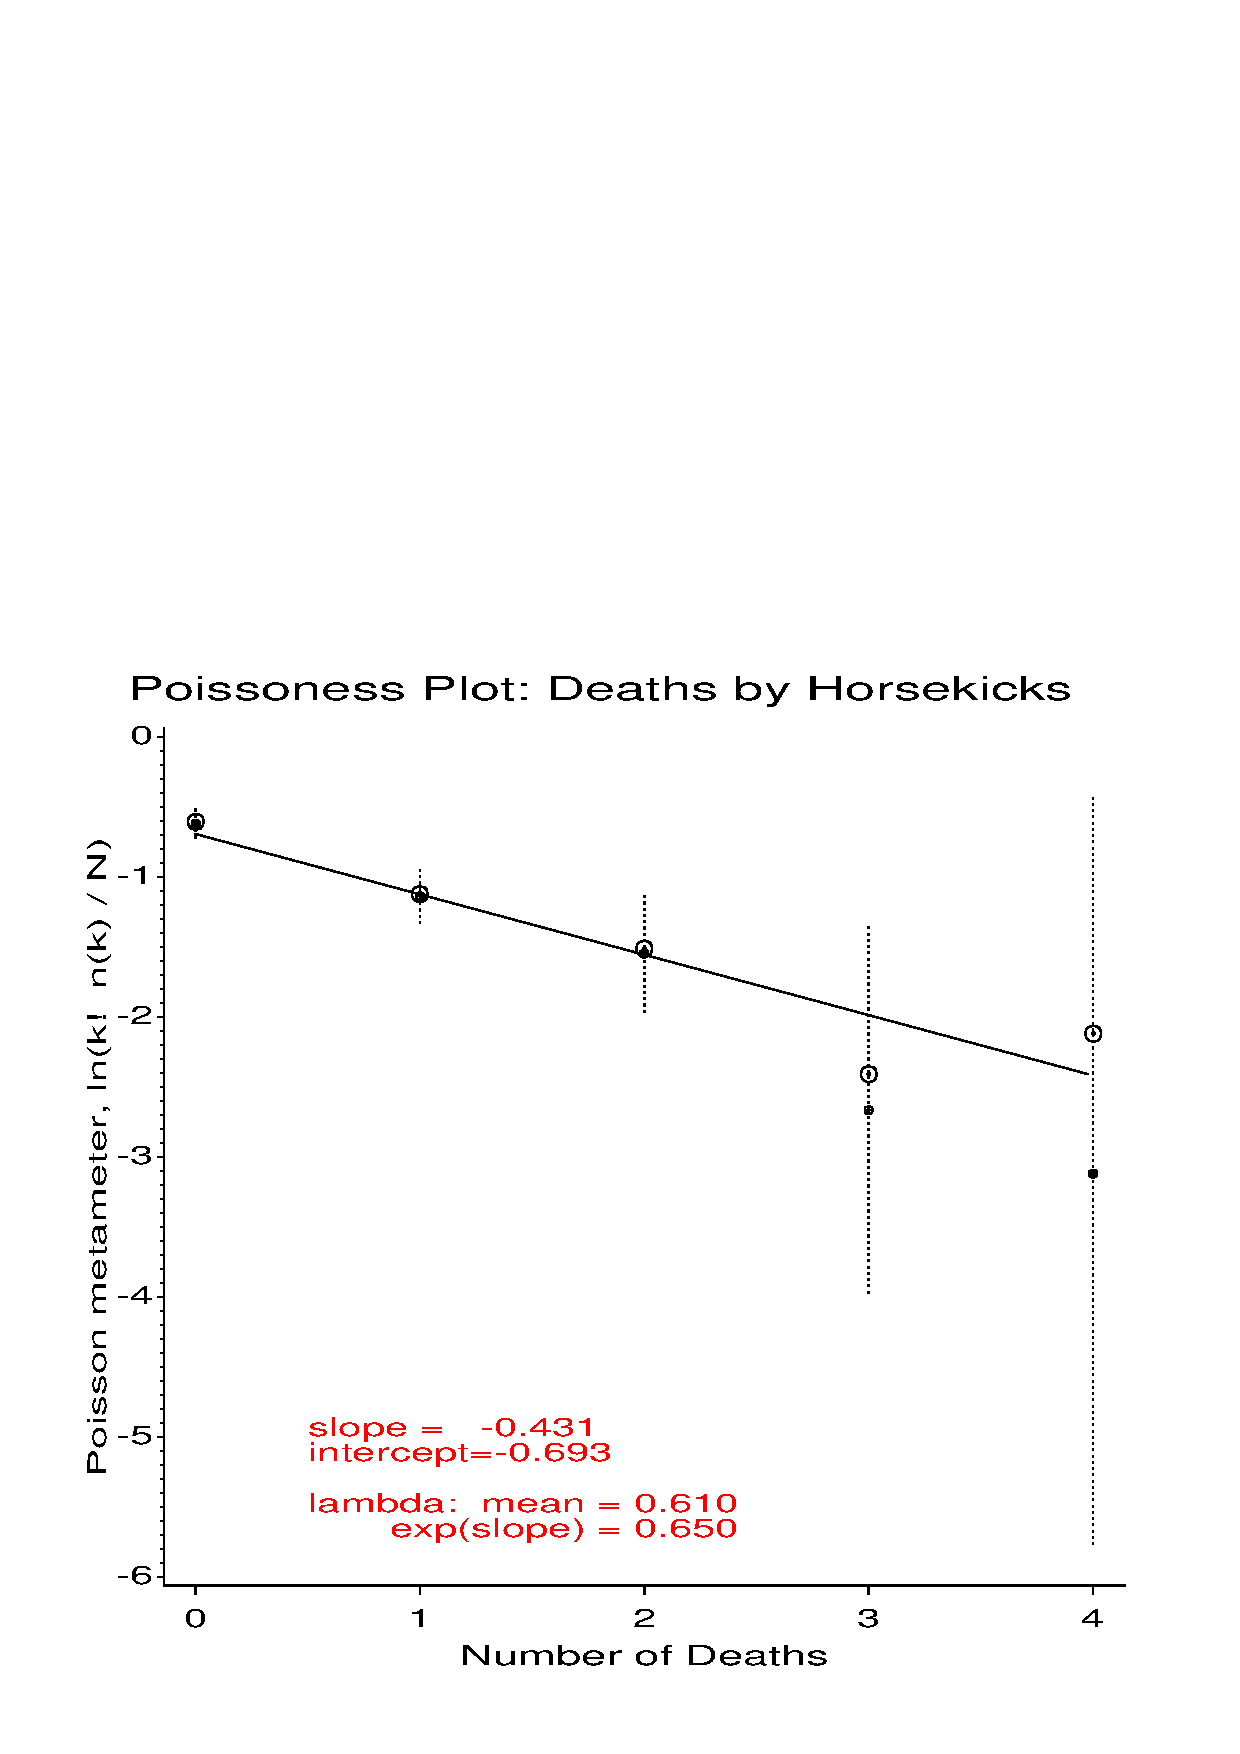
\includegraphics[width=1\linewidth]{poisdemo1}\graphicsfile{ch2/fig/poisdemo1.eps}{}
 \end{minipage}
\end{center}

   %% visual contents images

\chapterprelude{
Creating and manipulating categorical data sets requires
some skills and techniques in \R beyond those ordinarily used
for quantitative data. This chapter illustrates these for the
main formats for categorical data: case form, frequency form
and table form.
}

\DONE{DM: The chapter does not cover NA handling, although this is needed
  in some chapters. Maybe treat this in the also missing section on
  subsetting? --- The note for \code{table} and in the subsetting
  section should suffice.}

Categorical data can be represented as data sets
in various formats:
case form, frequency form, and table form.  This chapter
describes and illustrates the skills and techniques in \R
needed to input, create and manipulate \R data objects
to represent categorical data, and convert these from one
form to another for the purposes of statistical analysis
and visualization which are the subject of the remainder of the book.

As mentioned earlier, this book assumes that you have at least a
basic knowledge of the \R language and environment, including
interacting with the \R console (Rgui for Windows, R.app for Mac OS X)
or some other editor/environment (e.g., R Studio),
loading and using \R functions in packages (e.g., \code{library(vcd)})
getting help for these from \R (e.g., \code{help(matrix)}), etc.
This chapter is therefore devoted
to covering those topics beyond such basic skills needed in the book.%
\footnote{
Some excellent introductory treatments of \R are:
\citet[\C 2]{FoxWeisberg:2011}, ...
Tom Short's \emph{R Reference Card}, \url{http://cran.us.r-project.org/doc/contrib/Short-refcard.pdf} is a handy 4-page summary of the main functions.
The web sites
Quick-R \url{http://www.statmethods.net/} and
Cookbook for R \url{http://www.cookbook-r.com/}
provide very helpful examples, organized by topics and tasks.
}


\section{Working with \R data: vectors, matrices, arrays and data frames}\label{sec:Rdata}

\R has a wide variety of data structures for storing, manipulating and
calculating with data.  Among these, vectors, matrices, arrays and
data frames are most important for the material in this book.

In \R, a \term{vector} is a collection of values, like numbers,
character strings, or logicals (\code{TRUE, FALSE}), and often correspond to a variable in some analysis.
Matrices are rectangular arrays like a traditional table, composed of vectors in their columns
or rows.
Arrays add additional dimensions, so that, for example, a 3-way table can be represented
as composed of rows, columns and layers.
An important consideration is that the values in vectors,
matrices and arrays must all be of the same \emph{mode}, e.g., numbers or character strings.
A \term{data frame} is a rectangular table, like a traditional data set in other
statistical environments, and composed of rows and columns like a matrix,
but allowing variables (columns) of different types. These data structures and the types of
data they can contain are illustrated in \figref{fig:datatypes}. A more general
data structure is a \emph{list}, a generic vector which can contain
any other types of objects (including lists, allowing for \emph{recursive}
data structures). A data frame is basically a list of equally-sized
vectors, each representing a column of the data frame.

\begin{figure}
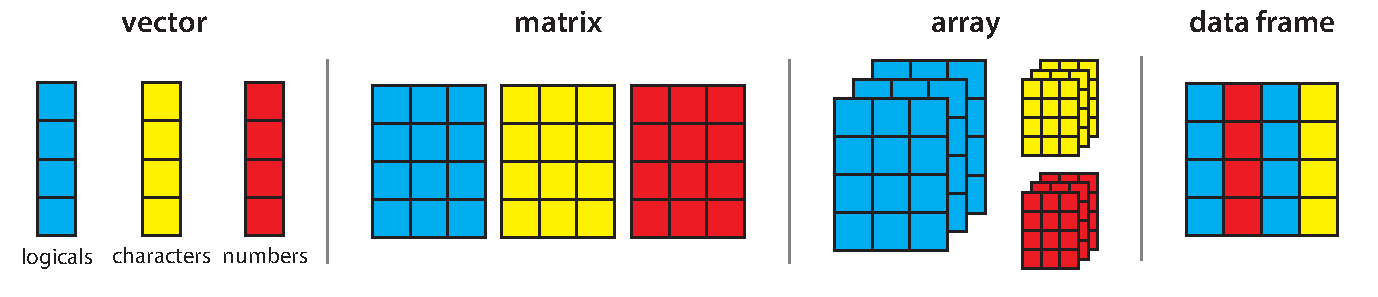
\includegraphics[width=\textwidth]{ch02/fig/datatypes2}
\caption[Principal data structures and data types in R]{Principal data structures and data types in \R. Colors
 represent different data types: numeric, character, logical. }
\label{fig:datatypes}
\end{figure}

\TODO{Delete subsections on vectors, matrices and arrays?}

\subsection{Vectors}
The simplest data structure in \R is a \term{vector}, a one-dimensional
collection of elements of the same type. An easy way to create a vector is with
the \func{c}, which combines its arguments.  The following examples create
and print vectors of length 4, containing numbers, character strings and
logical values respectively:

\begin{knitrout}
\definecolor{shadecolor}{rgb}{1, 0.961, 0.933}\color{fgcolor}\begin{kframe}
\begin{alltt}
\hlstd{> }\hlkwd{c}\hlstd{(}\hlnum{17}\hlstd{,} \hlnum{20}\hlstd{,} \hlnum{15}\hlstd{,} \hlnum{40}\hlstd{)}
\end{alltt}
\begin{verbatim}
[1] 17 20 15 40
\end{verbatim}
\begin{alltt}
\hlstd{> }\hlkwd{c}\hlstd{(}\hlstr{"female"}\hlstd{,} \hlstr{"male"}\hlstd{,} \hlstr{"female"}\hlstd{,} \hlstr{"male"}\hlstd{)}
\end{alltt}
\begin{verbatim}
[1] "female" "male"   "female" "male"  
\end{verbatim}
\begin{alltt}
\hlstd{> }\hlkwd{c}\hlstd{(}\hlnum{TRUE}\hlstd{,} \hlnum{TRUE}\hlstd{,} \hlnum{FALSE}\hlstd{,} \hlnum{FALSE}\hlstd{)}
\end{alltt}
\begin{verbatim}
[1]  TRUE  TRUE FALSE FALSE
\end{verbatim}
\end{kframe}
\end{knitrout}

To store these values in variables, \R uses the assignment operator (\code{<-})
or equals sign (\code{=}). This creates a variable named on the left-hand side.
An assignment doesn't print the result, but a bare expression does, so you can
assign and print by surrounding the assignment with \code{()}.

\begin{knitrout}
\definecolor{shadecolor}{rgb}{1, 0.961, 0.933}\color{fgcolor}\begin{kframe}
\begin{alltt}
\hlstd{> }\hlstd{count} \hlkwb{<-} \hlkwd{c}\hlstd{(}\hlnum{17}\hlstd{,} \hlnum{20}\hlstd{,} \hlnum{15}\hlstd{,} \hlnum{40}\hlstd{)}                       \hlcom{# assign}
\hlstd{> }\hlstd{count}                                            \hlcom{# print}
\end{alltt}
\begin{verbatim}
[1] 17 20 15 40
\end{verbatim}
\begin{alltt}
\hlstd{> }\hlstd{(sex} \hlkwb{<-} \hlkwd{c}\hlstd{(}\hlstr{"female"}\hlstd{,} \hlstr{"male"}\hlstd{,} \hlstr{"female"}\hlstd{,} \hlstr{"male"}\hlstd{))}   \hlcom{# both}
\end{alltt}
\begin{verbatim}
[1] "female" "male"   "female" "male"  
\end{verbatim}
\begin{alltt}
\hlstd{> }\hlstd{(passed} \hlkwb{<-} \hlkwd{c}\hlstd{(}\hlnum{TRUE}\hlstd{,} \hlnum{TRUE}\hlstd{,} \hlnum{FALSE}\hlstd{,} \hlnum{FALSE}\hlstd{))}
\end{alltt}
\begin{verbatim}
[1]  TRUE  TRUE FALSE FALSE
\end{verbatim}
\end{kframe}
\end{knitrout}

Other useful functions for creating vectors are:
\begin{itemize*}
  \item The \code{:} operator for generating consecutive integer sequences, e.g.,
  \code{1:10} gives the integers 1 to 10.  The \func{seq} function is more general, taking the forms
\code{seq(from, to)},
\code{seq(from, to, by= )}, and
\code{seq(from, to, length= )} where the optional argument \code{by} specifies the interval between adjacent values and \code{length} gives the desired length of the
result.

  \item The \func{rep} function generates repeated sequences, replicating
  its first argument (which may be a vector) a given number of \code{times},
  to a given \code{length} or \code{each} a given multiple.
\end{itemize*}

\begin{knitrout}
\definecolor{shadecolor}{rgb}{1, 0.961, 0.933}\color{fgcolor}\begin{kframe}
\begin{alltt}
\hlstd{> }\hlkwd{seq}\hlstd{(}\hlnum{10}\hlstd{,} \hlnum{100}\hlstd{,} \hlkwc{by} \hlstd{=} \hlnum{10}\hlstd{)}      \hlcom{# give interval}
\end{alltt}
\begin{verbatim}
 [1]  10  20  30  40  50  60  70  80  90 100
\end{verbatim}
\begin{alltt}
\hlstd{> }\hlkwd{seq}\hlstd{(}\hlnum{0}\hlstd{,} \hlnum{1}\hlstd{,} \hlkwc{length} \hlstd{=} \hlnum{11}\hlstd{)}     \hlcom{# give length}
\end{alltt}
\begin{verbatim}
 [1] 0.0 0.1 0.2 0.3 0.4 0.5 0.6 0.7 0.8 0.9 1.0
\end{verbatim}
\begin{alltt}
\hlstd{> }\hlstd{(sex} \hlkwb{<-} \hlkwd{rep}\hlstd{(}\hlkwd{c}\hlstd{(}\hlstr{"female"}\hlstd{,} \hlstr{"male"}\hlstd{),} \hlkwc{times} \hlstd{=} \hlnum{2}\hlstd{))}
\end{alltt}
\begin{verbatim}
[1] "female" "male"   "female" "male"  
\end{verbatim}
\begin{alltt}
\hlstd{> }\hlstd{(sex} \hlkwb{<-} \hlkwd{rep}\hlstd{(}\hlkwd{c}\hlstd{(}\hlstr{"female"}\hlstd{,} \hlstr{"male"}\hlstd{),} \hlkwc{length.out} \hlstd{=} \hlnum{4}\hlstd{))}  \hlcom{# same}
\end{alltt}
\begin{verbatim}
[1] "female" "male"   "female" "male"  
\end{verbatim}
\begin{alltt}
\hlstd{> }\hlstd{(passed} \hlkwb{<-} \hlkwd{rep}\hlstd{(}\hlkwd{c}\hlstd{(}\hlnum{TRUE}\hlstd{,} \hlnum{FALSE}\hlstd{),} \hlkwc{each} \hlstd{=} \hlnum{2}\hlstd{))}
\end{alltt}
\begin{verbatim}
[1]  TRUE  TRUE FALSE FALSE
\end{verbatim}
\end{kframe}
\end{knitrout}

\subsection{Matrices}
A \term{matrix} is a two-dimensional array of elements of the same type composed
in a rectangular array of rows and columns. Matrices can be created by the function
\code{matrix(values, nrow, ncol)}, which reshapes the elements in
the first argument (\code{values}) to a matrix with \code{nrow} rows and
\code{ncol} columns. By default, the elements are filled in columnwise, unless
the optional argument \code{byrow = TRUE} is given.

\begin{knitrout}
\definecolor{shadecolor}{rgb}{1, 0.961, 0.933}\color{fgcolor}\begin{kframe}
\begin{alltt}
\hlstd{> }\hlstd{(matA} \hlkwb{<-} \hlkwd{matrix}\hlstd{(}\hlnum{1}\hlopt{:}\hlnum{8}\hlstd{,} \hlkwc{nrow} \hlstd{=} \hlnum{2}\hlstd{,} \hlkwc{ncol} \hlstd{=} \hlnum{4}\hlstd{))}
\end{alltt}
\begin{verbatim}
     [,1] [,2] [,3] [,4]
[1,]    1    3    5    7
[2,]    2    4    6    8
\end{verbatim}
\begin{alltt}
\hlstd{> }\hlstd{(matB} \hlkwb{<-} \hlkwd{matrix}\hlstd{(}\hlnum{1}\hlopt{:}\hlnum{8}\hlstd{,} \hlkwc{nrow} \hlstd{=} \hlnum{2}\hlstd{,} \hlkwc{ncol} \hlstd{=} \hlnum{4}\hlstd{,} \hlkwc{byrow} \hlstd{=} \hlnum{TRUE}\hlstd{))}
\end{alltt}
\begin{verbatim}
     [,1] [,2] [,3] [,4]
[1,]    1    2    3    4
[2,]    5    6    7    8
\end{verbatim}
\begin{alltt}
\hlstd{> }\hlstd{(matC} \hlkwb{<-} \hlkwd{matrix}\hlstd{(}\hlnum{1}\hlopt{:}\hlnum{4}\hlstd{,} \hlkwc{nrow} \hlstd{=} \hlnum{2}\hlstd{,} \hlkwc{ncol} \hlstd{=} \hlnum{4}\hlstd{))}
\end{alltt}
\begin{verbatim}
     [,1] [,2] [,3] [,4]
[1,]    1    3    1    3
[2,]    2    4    2    4
\end{verbatim}
\end{kframe}
\end{knitrout}
\noindent The last example illustrates that the values in the first argument are recycled
as necessary to fill the given number of rows and columns.

All matrices have a dimensions attribute, a vector of length two giving the number
of rows and columns, retrieved with the function \func{dim}. Labels for the rows and
columns can be assigned using \func{dimnames},%
\footnote{
The \code{dimnames} can also be specified as an optional argument to \func{matrix}.
}
which takes a list of two vectors for the
row names and column names respectively. To see the structure of a matrix
(or any other \R object) and its attributes, you can
use the \func{str} function, as shown in the example below.

\begin{knitrout}
\definecolor{shadecolor}{rgb}{1, 0.961, 0.933}\color{fgcolor}\begin{kframe}
\begin{alltt}
\hlstd{> }\hlkwd{dim}\hlstd{(matA)}
\end{alltt}
\begin{verbatim}
[1] 2 4
\end{verbatim}
\begin{alltt}
\hlstd{> }\hlkwd{str}\hlstd{(matA)}
\end{alltt}
\begin{verbatim}
 int [1:2, 1:4] 1 2 3 4 5 6 7 8
\end{verbatim}
\begin{alltt}
\hlstd{> }\hlkwd{dimnames}\hlstd{(matA)} \hlkwb{<-} \hlkwd{list}\hlstd{(}\hlkwd{c}\hlstd{(}\hlstr{"M"}\hlstd{,} \hlstr{"F"}\hlstd{), LETTERS[}\hlnum{1}\hlopt{:}\hlnum{4}\hlstd{])}
\hlstd{> }\hlstd{matA}
\end{alltt}
\begin{verbatim}
  A B C D
M 1 3 5 7
F 2 4 6 8
\end{verbatim}
\begin{alltt}
\hlstd{> }\hlkwd{str}\hlstd{(matA)}
\end{alltt}
\begin{verbatim}
 int [1:2, 1:4] 1 2 3 4 5 6 7 8
 - attr(*, "dimnames")=List of 2
  ..$ : chr [1:2] "M" "F"
  ..$ : chr [1:4] "A" "B" "C" "D"
\end{verbatim}
\end{kframe}
\end{knitrout}
Additionally, names for the row and column \emph{variables} themselves can also be assigned in the
\code{dimnames} call by giving each dimension vector a name.
\begin{knitrout}
\definecolor{shadecolor}{rgb}{1, 0.961, 0.933}\color{fgcolor}\begin{kframe}
\begin{alltt}
\hlstd{> }\hlkwd{dimnames}\hlstd{(matA)} \hlkwb{<-} \hlkwd{list}\hlstd{(}\hlkwc{sex} \hlstd{=} \hlkwd{c}\hlstd{(}\hlstr{"M"}\hlstd{,} \hlstr{"F"}\hlstd{),} \hlkwc{group} \hlstd{= LETTERS[}\hlnum{1}\hlopt{:}\hlnum{4}\hlstd{])}
\hlstd{> }\hlcom{## or: names(dimnames(matA)) <- c("Sex", "Group")}
\hlstd{> }\hlstd{matA}
\end{alltt}
\begin{verbatim}
   group
sex A B C D
  M 1 3 5 7
  F 2 4 6 8
\end{verbatim}
\begin{alltt}
\hlstd{> }\hlkwd{str}\hlstd{(matA)}
\end{alltt}
\begin{verbatim}
 int [1:2, 1:4] 1 2 3 4 5 6 7 8
 - attr(*, "dimnames")=List of 2
  ..$ sex  : chr [1:2] "M" "F"
  ..$ group: chr [1:4] "A" "B" "C" "D"
\end{verbatim}
\end{kframe}
\end{knitrout}
\noindent (\code{LETTERS} is a predefined character 
vector of the 26 uppercase letters).
Matrices can also be created or enlarged by ``binding'' vectors or matrices together
by rows or columns:
\begin{itemize*}
  \item \code{rbind(a, b, c)} creates a matrix with the vectors \code{a}, \code{b} and \code{c} as its rows, recycling the elements as necessary to the length of the longest one.
  \item \code{cbind(a, b, c)} creates a matrix with the vectors \code{a}, \code{b} and \code{c} as its columns.
  \item \code{rbind(mat, a, b, ...)} and \code{cbind(mat, a, b, ...)} add additional
  rows (columns) to a matrix \code{mat}, recycling or subsetting the elements in the
  vectors to conform with the size of the matrix.
\end{itemize*}

\begin{knitrout}
\definecolor{shadecolor}{rgb}{1, 0.961, 0.933}\color{fgcolor}\begin{kframe}
\begin{alltt}
\hlstd{> }\hlkwd{rbind}\hlstd{(matA,} \hlkwd{c}\hlstd{(}\hlnum{10}\hlstd{,} \hlnum{20}\hlstd{))}
\end{alltt}
\begin{verbatim}
   A  B  C  D
M  1  3  5  7
F  2  4  6  8
  10 20 10 20
\end{verbatim}
\begin{alltt}
\hlstd{> }\hlkwd{cbind}\hlstd{(matA,} \hlkwd{c}\hlstd{(}\hlnum{10}\hlstd{,} \hlnum{20}\hlstd{))}
\end{alltt}
\begin{verbatim}
  A B C D   
M 1 3 5 7 10
F 2 4 6 8 20
\end{verbatim}
\end{kframe}
\end{knitrout}

\noindent Rows and columns can be swapped (transposed)
using \func{t}:

\begin{knitrout}
\definecolor{shadecolor}{rgb}{1, 0.961, 0.933}\color{fgcolor}\begin{kframe}
\begin{alltt}
\hlstd{> }\hlkwd{t}\hlstd{(matA)}
\end{alltt}
\begin{verbatim}
     sex
group M F
    A 1 2
    B 3 4
    C 5 6
    D 7 8
\end{verbatim}
\end{kframe}
\end{knitrout}

\noindent Finally, we note that basic computations involving matrices
are performed \emph{element-wise}:

\begin{knitrout}
\definecolor{shadecolor}{rgb}{1, 0.961, 0.933}\color{fgcolor}\begin{kframe}
\begin{alltt}
\hlstd{> }\hlnum{2} \hlopt{*} \hlstd{matA} \hlopt{/} \hlnum{100}
\end{alltt}
\begin{verbatim}
   group
sex    A    B    C    D
  M 0.02 0.06 0.10 0.14
  F 0.04 0.08 0.12 0.16
\end{verbatim}
\end{kframe}
\end{knitrout}

\noindent Special operators and functions do exist for matrix
operations, such as \code{\%*\%} for the matrix product. %

\subsection{Arrays}
Higher-dimensional arrays are less frequently encountered in traditional data analysis,
but they are of great use for categorical data, where frequency tables of three or more
variables can be naturally represented as arrays, with one dimension for each
table variable.

The function \code{array(values, dim)} takes the elements in \code{values} and
reshapes these into an array whose dimensions are given in the vector \code{dim}.
The number of dimensions is the length of \code{dim}.  As with matrices, the
elements are filled in with the first dimension (rows) varying most rapidly,
then by the second dimension (columns) and so on for all further dimensions,
which can be considered as layers.
A matrix is just the special case of an array with two dimensions.

\begin{knitrout}
\definecolor{shadecolor}{rgb}{1, 0.961, 0.933}\color{fgcolor}\begin{kframe}
\begin{alltt}
\hlstd{> }\hlstd{(arrayA} \hlkwb{<-} \hlkwd{array}\hlstd{(}\hlnum{1}\hlopt{:}\hlnum{16}\hlstd{,} \hlkwc{dim} \hlstd{=} \hlkwd{c}\hlstd{(}\hlnum{2}\hlstd{,} \hlnum{4}\hlstd{,} \hlnum{2}\hlstd{)))}     \hlcom{# 2 rows, 4 columns, 2 layers}
\end{alltt}
\begin{verbatim}
, , 1

     [,1] [,2] [,3] [,4]
[1,]    1    3    5    7
[2,]    2    4    6    8

, , 2

     [,1] [,2] [,3] [,4]
[1,]    9   11   13   15
[2,]   10   12   14   16
\end{verbatim}
\begin{alltt}
\hlstd{> }\hlkwd{str}\hlstd{(arrayA)}
\end{alltt}
\begin{verbatim}
 int [1:2, 1:4, 1:2] 1 2 3 4 5 6 7 8 9 10 ...
\end{verbatim}
\begin{alltt}
\hlstd{> }\hlstd{(arrayB} \hlkwb{<-} \hlkwd{array}\hlstd{(}\hlnum{1}\hlopt{:}\hlnum{16}\hlstd{,} \hlkwc{dim} \hlstd{=} \hlkwd{c}\hlstd{(}\hlnum{2}\hlstd{,} \hlnum{8}\hlstd{)))}        \hlcom{# 2 rows, 8 columns}
\end{alltt}
\begin{verbatim}
     [,1] [,2] [,3] [,4] [,5] [,6] [,7] [,8]
[1,]    1    3    5    7    9   11   13   15
[2,]    2    4    6    8   10   12   14   16
\end{verbatim}
\begin{alltt}
\hlstd{> }\hlkwd{str}\hlstd{(arrayB)}
\end{alltt}
\begin{verbatim}
 int [1:2, 1:8] 1 2 3 4 5 6 7 8 9 10 ...
\end{verbatim}
\end{kframe}
\end{knitrout}
In the same way that we can assign labels to the rows, columns and variables
in matrices, we can assign these attributes to \code{dimnames(arrayA)}, or
include this information in a \code{dimnames=} argument to \func{array}.

\begin{knitrout}
\definecolor{shadecolor}{rgb}{1, 0.961, 0.933}\color{fgcolor}\begin{kframe}
\begin{alltt}
\hlstd{> }\hlkwd{dimnames}\hlstd{(arrayA)} \hlkwb{<-} \hlkwd{list}\hlstd{(}\hlkwc{sex} \hlstd{=} \hlkwd{c}\hlstd{(}\hlstr{"M"}\hlstd{,} \hlstr{"F"}\hlstd{),}
\hlstd{+ }                         \hlkwc{group} \hlstd{= letters[}\hlnum{1}\hlopt{:}\hlnum{4}\hlstd{],}
\hlstd{+ }                         \hlkwc{time} \hlstd{=} \hlkwd{c}\hlstd{(}\hlstr{"Pre"}\hlstd{,} \hlstr{"Post"}\hlstd{))}
\hlstd{> }\hlstd{arrayA}
\end{alltt}
\begin{verbatim}
, , time = Pre

   group
sex a b c d
  M 1 3 5 7
  F 2 4 6 8

, , time = Post

   group
sex  a  b  c  d
  M  9 11 13 15
  F 10 12 14 16
\end{verbatim}
\begin{alltt}
\hlstd{> }\hlkwd{str}\hlstd{(arrayA)}
\end{alltt}
\begin{verbatim}
 int [1:2, 1:4, 1:2] 1 2 3 4 5 6 7 8 9 10 ...
 - attr(*, "dimnames")=List of 3
  ..$ sex  : chr [1:2] "M" "F"
  ..$ group: chr [1:4] "a" "b" "c" "d"
  ..$ time : chr [1:2] "Pre" "Post"
\end{verbatim}
\end{kframe}
\end{knitrout}

Arrays in \R can contain any single type of elements--- numbers,
character strings, logicals.  \R also has a variety of functions
(e.g., \func{table}, \func{xtabs})
for creating and manipulating \class{table} objects, which are
specialized forms of matrices and arrays containing integer
frequencies in a contingency table. These are discussed in more
detail below (\secref{sec:table}).


\subsection{data frames}\label{sec:data-frames}
Data frames are the most commonly used form of data in \R and more
general than matrices in that they can contain columns of different types.
For statistical modeling, data frames play a special role, in that
many modeling functions are designed to take a data frame as a
\code{data=} argument, and then find the variables mentioned within
that data frame. Another distinguishing feature is that discrete variables
(columns) like character strings \code{("M", "F")} or integers \code{(1, 2, 3)}
in data frames can be represented as \term{factor}s, which simplifies
many statistical and graphical methods.

A data frame can be created using keyboard input
with the \func{data.frame} function, applied to a list of objects,
\code{data.frame(a, b, c, ...)}, each of which can be a vector, matrix or another
data frame, but typically all containing the same number of rows.
This works roughly like \func{cbind}, collecting the arguments as columns
in the result.

The following example generates \code{n = 100} random observations on
three discrete factor variables, \code{A, B, sex}, and a numeric
variable, \code{age}.  As constructed, all of these are
statistically independent, since none depends on any of the others.
The function \func{sample}
is used here to generate \code{n} random samples from the
first argument allowing replacement (\code{replace = TRUE}).
The \func{rnorm()} function produces a vector of \code{n} normally
distributed values with mean 30 and standard deviation 5.
The call to \func{set.seed} guarantees the reproducibility of the
resulting data. 
Finally, all four variables are combined into the data frame
\code{mydata}.


\begin{knitrout}
\definecolor{shadecolor}{rgb}{1, 0.961, 0.933}\color{fgcolor}\begin{kframe}
\begin{alltt}
\hlstd{> }\hlkwd{set.seed}\hlstd{(}\hlnum{12345}\hlstd{)}   \hlcom{# reproducibility}
\hlstd{> }\hlstd{n} \hlkwb{<-} \hlnum{100}
\hlstd{> }\hlstd{A} \hlkwb{<-} \hlkwd{factor}\hlstd{(}\hlkwd{sample}\hlstd{(}\hlkwd{c}\hlstd{(}\hlstr{"a1"}\hlstd{,} \hlstr{"a2"}\hlstd{), n,} \hlkwc{replace} \hlstd{=} \hlnum{TRUE}\hlstd{))}
\hlstd{> }\hlstd{B} \hlkwb{<-} \hlkwd{factor}\hlstd{(}\hlkwd{sample}\hlstd{(}\hlkwd{c}\hlstd{(}\hlstr{"b1"}\hlstd{,} \hlstr{"b2"}\hlstd{), n,} \hlkwc{replace} \hlstd{=} \hlnum{TRUE}\hlstd{))}
\hlstd{> }\hlstd{sex} \hlkwb{<-} \hlkwd{factor}\hlstd{(}\hlkwd{sample}\hlstd{(}\hlkwd{c}\hlstd{(}\hlstr{"M"}\hlstd{,} \hlstr{"F"}\hlstd{), n,} \hlkwc{replace} \hlstd{=} \hlnum{TRUE}\hlstd{))}
\hlstd{> }\hlstd{age} \hlkwb{<-} \hlkwd{round}\hlstd{(}\hlkwd{rnorm}\hlstd{(n,} \hlkwc{mean} \hlstd{=} \hlnum{30}\hlstd{,} \hlkwc{sd} \hlstd{=} \hlnum{5}\hlstd{))}
\hlstd{> }\hlstd{mydata} \hlkwb{<-} \hlkwd{data.frame}\hlstd{(A, B, sex, age)}
\hlstd{> }\hlkwd{head}\hlstd{(mydata,} \hlnum{5}\hlstd{)}
\end{alltt}
\begin{verbatim}
   A  B sex age
1 a2 b1   F  22
2 a2 b2   F  33
3 a2 b2   M  31
4 a2 b2   F  26
5 a1 b2   F  29
\end{verbatim}
\begin{alltt}
\hlstd{> }\hlkwd{str}\hlstd{(mydata)}
\end{alltt}
\begin{verbatim}
'data.frame':	100 obs. of  4 variables:
 $ A  : Factor w/ 2 levels "a1","a2": 2 2 2 2 1 1 1 2 2 2 ...
 $ B  : Factor w/ 2 levels "b1","b2": 1 2 2 2 2 2 2 2 1 1 ...
 $ sex: Factor w/ 2 levels "F","M": 1 1 2 1 1 1 2 2 1 1 ...
 $ age: num  22 33 31 26 29 29 38 28 30 27 ...
\end{verbatim}
\end{kframe}
\end{knitrout}

Rows, columns and individual values in a data frame can be manipulated
in the same way as a matrix. Additionally, variables can be extracted
using the \code{$} operator:

\begin{knitrout}
\definecolor{shadecolor}{rgb}{1, 0.961, 0.933}\color{fgcolor}\begin{kframe}
\begin{alltt}
\hlstd{> }\hlstd{mydata[}\hlnum{1}\hlstd{,}\hlnum{2}\hlstd{]}
\end{alltt}
\begin{verbatim}
[1] b1
Levels: b1 b2
\end{verbatim}
\begin{alltt}
\hlstd{> }\hlstd{mydata}\hlopt{$}\hlstd{sex}
\end{alltt}
\begin{verbatim}
  [1] F F M F F F M M F F M F M M F M M F F M M M M F F F F M M F
 [31] M F M F F F F F M M F F F F F F F F M F M F M M F F M M M M
 [61] F F F F F M M F F F M M M F F M F M M F M F M M M M M F F F
 [91] F F M M F M F M F M
Levels: F M
\end{verbatim}
\begin{alltt}
\hlstd{> }\hlcom{##same as: mydata[,"sex"] or mydata[,3]}
\end{alltt}
\end{kframe}
\end{knitrout}
\noindent Values in data frames can conveniently be edited using,
e.g., \code{fix(mydata)}, opening a simple, spreadsheet-like editor.

For real data sets, it is usually most convenient to read these into \R
from external files, and this is easiest using plain text (ASCII) files
with one line per observation and fields separated by commas (or tabs),
and with a first header line giving the variable names-- called
\emph{comma-separated} or CSV format.
If your data is in the form of Excel, SAS, SPSS or other file format,
you can almost always export that data to CSV format first.%
\footnote{
The \Rpackage{foreign} contains specialized functions to \emph{directly} read
data stored by Minitab, SAS, SPSS, Stata, Systat and other software.
There are also a number of packages for reading (and writing)
Excel spreadsheets directly (\pkg{gdata}, \pkg{XLConnect}, \pkg{xlsx}).
The \R manual, \emph{R Data Import/Export} covers many other variations,
including data in relational data bases.
}

The function \func{read.table} has many options to control the details
of how the data are read and converted to variables in the data frame.
Among these some important options are:
\begin{description*}
  \item [\code{header}] indicates whether the first line contains
variable names. The default is \code{FALSE} unless the first line contains one fewer field
than the number of columns;
  \item[\code{sep}] (default: \code{""} meaning white space, i.e., one or more spaces, tabs or newlines) specifies the separator character between fields;
  \item[\code{stringsAsFactors}] (default: \code{TRUE}) determines whether character string variables should be converted to factors;
  \item[\code{na.strings}] (default: \code{"NA"}) one or more strings which are interpreted
  as missing data values (\code{NA});
\end{description*}
For delimited files, \func{read.csv} and \func{read.delim} are convenient wrappers
to \func{read.table}, with default values \code{sep=","} and \code{sep="\t"}
respectively, and
\code{header=TRUE}.

\begin{Example}[ch2-arth-csv]{Arthritis treatment}

The file \code{Arthritis.csv} contains data in CSV format
from \citet{KochEdwards:88}, representing
a double-blind clinical trial investigating a new treatment for rheumatoid arthritis with 84 patients.
\footnote{This data can be created using: \code{library(vcd); write.table(Arthritis, file = "Arthritis.csv", quote = FALSE, sep = ",")} }
The first (``header'') line gives the variable names.  Some of the
lines in the file are shown below, with \code{...} representing omitted lines:
{\small
\renewcommand{\baselinestretch}{.85}
%<<arth-csv, eval=FALSE, results='asis'>>=
\begin{verbatim}
ID,Treatment,Sex,Age,Improved
57,Treated,Male,27,Some
46,Treated,Male,29,None
77,Treated,Male,30,None
17,Treated,Male,32,Marked
 ...
42,Placebo,Female,66,None
15,Placebo,Female,66,Some
71,Placebo,Female,68,Some
1,Placebo,Female,74,Marked
\end{verbatim}
%@
}

\DONE{DM: Add this to vcd or vcdExtra. --- added footnote.}

We read this into \R using \func{read.table} as shown below:
\begin{knitrout}\footnotesize
\definecolor{shadecolor}{rgb}{1, 0.961, 0.933}\color{fgcolor}\begin{kframe}
\begin{alltt}
\hlstd{> }\hlstd{path} \hlkwb{<-} \hlstr{"ch02/Arthritis.csv"} \hlcom{## set path}
\hlstd{> }\hlcom{## for convenience, use path <- file.choose() to retrieve a path }
\hlstd{> }\hlcom{## then, use file.show(path) to inspect the data format}
\hlstd{> }\hlstd{Arthritis} \hlkwb{<-} \hlkwd{read.table}\hlstd{(path,} \hlkwc{header} \hlstd{=} \hlnum{TRUE}\hlstd{,} \hlkwc{sep} \hlstd{=} \hlstr{","}\hlstd{)}
\hlstd{> }\hlkwd{str}\hlstd{(Arthritis)}
\end{alltt}
\begin{verbatim}
'data.frame':	84 obs. of  5 variables:
 $ ID       : int  57 46 77 17 36 23 75 39 33 55 ...
 $ Treatment: Factor w/ 2 levels "Placebo","Treated": 2 2 2 2 2 2 2 2 2 2 ...
 $ Sex      : Factor w/ 2 levels "Female","Male": 2 2 2 2 2 2 2 2 2 2 ...
 $ Age      : int  27 29 30 32 46 58 59 59 63 63 ...
 $ Improved : Factor w/ 3 levels "Marked","None",..: 3 2 2 1 1 1 2 1 2 2 ...
\end{verbatim}
\end{kframe}
\end{knitrout}
Note that the character variables \var{Treatment}, \var{Sex} and \var{Improved}
were converted to factors, and the levels of those variables were
ordered \emph{alphabetically}.  This often doesn't matter much for binary variables,
but here, the response variable, \var{Improved} has levels
that should be considered \emph{ordered},
as \code{"None", "Some", "Marked"}.  We can correct this here by
re-assigning \code{Arthritis$Improved} using \func{ordered}.
The topic of re-ordering variables and levels in categorical data is
considered in more detail in \secref{sec:ordered}.

\begin{knitrout}
\definecolor{shadecolor}{rgb}{1, 0.961, 0.933}\color{fgcolor}\begin{kframe}
\begin{alltt}
\hlstd{> }\hlkwd{levels}\hlstd{(Arthritis}\hlopt{$}\hlstd{Improved)}
\end{alltt}
\begin{verbatim}
[1] "Marked" "None"   "Some"  
\end{verbatim}
\begin{alltt}
\hlstd{> }\hlstd{Arthritis}\hlopt{$}\hlstd{Improved} \hlkwb{<-} \hlkwd{ordered}\hlstd{(Arthritis}\hlopt{$}\hlstd{Improved,}
\hlstd{+ }                              \hlkwc{levels} \hlstd{=} \hlkwd{c}\hlstd{(}\hlstr{"None"}\hlstd{,} \hlstr{"Some"}\hlstd{,} \hlstr{"Marked"}\hlstd{))}
\end{alltt}
\end{kframe}
\end{knitrout}

\end{Example}

\section{Forms of categorical data: case form, frequency form and table form}\label{sec:forms}
As we saw in \chref{ch:intro}, categorical data can be represented as ordinary data sets
in case form, but the discrete nature of factors or stratifying variables allows the same
information to be represented more compactly in summarized form with a frequency
variable for each cell of factor combinations, or in tables.
Consequently, we sometimes
find data created or presented in one form (e.g., a spreadsheet data set, a two-way
table of frequencies) and want to input that into \R.  Once we have the data in \R,
it is often necessary to manipulate the data into some other form for the purposes
of statistical analysis, visualizing results and our own presentation.
It is useful to understand the three main forms of categorical data in \R and how
to work with them for our purposes.

\subsection{Case form}
Categorical data in case form are simply data frames, with one or more discrete
classifying variables or response variables, most conveniently represented as factors or ordered factors.  In case form, the data set can also contain numeric variables
(covariates or other response variables), that cannot be accommodated in other
forms.

As with any data frame, \code{X}, you can access or compute with its attributes using \code{nrow(X)} for the number of observations,
\code{ncol(X)} for the number of variables,
\code{names(X)} or \code{colnames(X)} for the variable names and
so forth.

\begin{Example}[ch2-arth]{Arthritis treatment}

The \data{Arthritis} data is available in case form in the \pkg{vcd} package.
There are two explanatory factors: \code{Treatment} and \code{Sex}. \code{Age}
is a numeric covariate, and \code{Improved} is the response---an ordered factor,
with levels
%\code{paste(levels(Arthritis$Improved),collapse=' < ')}.
\code{"None" < "Some" < "Marked"}. Excluding \code{Age}, we would have
a $2 \times 2 \times 3$ contingency table for \code{Treatment}, \code{Sex} and \code{Improved}.
\begin{knitrout}\footnotesize
\definecolor{shadecolor}{rgb}{1, 0.961, 0.933}\color{fgcolor}\begin{kframe}
\begin{alltt}
\hlstd{> }\hlkwd{data}\hlstd{(Arthritis,} \hlkwc{package} \hlstd{=} \hlstr{"vcd"}\hlstd{)}  \hlcom{# load the data}
\hlstd{> }\hlkwd{names}\hlstd{(Arthritis)}      \hlcom{# show the variables}
\end{alltt}
\begin{verbatim}
[1] "ID"        "Treatment" "Sex"       "Age"       "Improved" 
\end{verbatim}
\begin{alltt}
\hlstd{> }\hlkwd{str}\hlstd{(Arthritis)}        \hlcom{# show the structure}
\end{alltt}
\begin{verbatim}
'data.frame':	84 obs. of  5 variables:
 $ ID       : int  57 46 77 17 36 23 75 39 33 55 ...
 $ Treatment: Factor w/ 2 levels "Placebo","Treated": 2 2 2 2 2 2 2 2 2 2 ...
 $ Sex      : Factor w/ 2 levels "Female","Male": 2 2 2 2 2 2 2 2 2 2 ...
 $ Age      : int  27 29 30 32 46 58 59 59 63 63 ...
 $ Improved : Ord.factor w/ 3 levels "None"<"Some"<..: 2 1 1 3 3 3 1 3 1 1 ...
\end{verbatim}
\begin{alltt}
\hlstd{> }\hlkwd{head}\hlstd{(Arthritis,} \hlnum{5}\hlstd{)}    \hlcom{# first 5 observations, same as Arthritis[1:5,]}
\end{alltt}
\begin{verbatim}
  ID Treatment  Sex Age Improved
1 57   Treated Male  27     Some
2 46   Treated Male  29     None
3 77   Treated Male  30     None
4 17   Treated Male  32   Marked
5 36   Treated Male  46   Marked
\end{verbatim}
\end{kframe}
\end{knitrout}
\end{Example}

\subsection{Frequency form}
Data in frequency form is also a data frame, containing
one or more discrete factor variables and a frequency variable
(often called \code{Freq} or \code{count})
representing the number of basic observations in that cell.

This is an alternative representation of a table form data set considered
below.
In frequency form, the number of cells in the equivalent table
is \code{nrow(X)}, and the total number of observations
is the sum of the frequency variable, \code{sum(X$Freq)}, %$
 \code{sum(X[,"Freq"])} or a similar expression.

\begin{Example}[ch2-GSS]{General social survey}
For small frequency tables, it is often convenient to enter them in frequency form
using \func{expand.grid} for the factors and \func{c} to list the counts in a vector.
The example below, from \cite{Agresti:2002} gives results for the 1991 General Social Survey,
with respondents classified by sex and party identification.
As a table, the data look like this:
\begin{center}
\begin{tabular}{rrrr}
  \hline
    &     & party & \\
  \hline
sex & dem & indep & rep \\
  \hline
female & 279 & 73 & 225 \\
  male & 165 & 47 & 191 \\
   \hline
\end{tabular}
\end{center}


We use \func{expand.grid} to create a $6 \times 2$ matrix
containing the combinations of \code{sex} and \code{party}
with the levels for \code{sex} given first, so that this varies
most rapidly. Then,
input the frequencies in the table by columns from
left to right, and combine these two results with
\func{data.frame}.
\begin{knitrout}
\definecolor{shadecolor}{rgb}{1, 0.961, 0.933}\color{fgcolor}\begin{kframe}
\begin{alltt}
\hlstd{> }\hlcom{# Agresti (2002), table 3.11, p. 106}
\hlstd{> }\hlstd{tmp} \hlkwb{<-} \hlkwd{expand.grid}\hlstd{(}\hlkwc{sex} \hlstd{=} \hlkwd{c}\hlstd{(}\hlstr{"female"}\hlstd{,} \hlstr{"male"}\hlstd{),}
\hlstd{+ }                   \hlkwc{party} \hlstd{=} \hlkwd{c}\hlstd{(}\hlstr{"dem"}\hlstd{,} \hlstr{"indep"}\hlstd{,} \hlstr{"rep"}\hlstd{))}
\hlstd{> }\hlstd{tmp}
\end{alltt}
\begin{verbatim}
     sex party
1 female   dem
2   male   dem
3 female indep
4   male indep
5 female   rep
6   male   rep
\end{verbatim}
\begin{alltt}
\hlstd{> }\hlstd{GSS} \hlkwb{<-} \hlkwd{data.frame}\hlstd{(tmp,} \hlkwc{count} \hlstd{=} \hlkwd{c}\hlstd{(}\hlnum{279}\hlstd{,} \hlnum{165}\hlstd{,} \hlnum{73}\hlstd{,} \hlnum{47}\hlstd{,} \hlnum{225}\hlstd{,} \hlnum{191}\hlstd{))}
\hlstd{> }\hlstd{GSS}
\end{alltt}
\begin{verbatim}
     sex party count
1 female   dem   279
2   male   dem   165
3 female indep    73
4   male indep    47
5 female   rep   225
6   male   rep   191
\end{verbatim}
\begin{alltt}
\hlstd{> }\hlkwd{names}\hlstd{(GSS)}
\end{alltt}
\begin{verbatim}
[1] "sex"   "party" "count"
\end{verbatim}
\begin{alltt}
\hlstd{> }\hlkwd{str}\hlstd{(GSS)}
\end{alltt}
\begin{verbatim}
'data.frame':	6 obs. of  3 variables:
 $ sex  : Factor w/ 2 levels "female","male": 1 2 1 2 1 2
 $ party: Factor w/ 3 levels "dem","indep",..: 1 1 2 2 3 3
 $ count: num  279 165 73 47 225 191
\end{verbatim}
\begin{alltt}
\hlstd{> }\hlkwd{sum}\hlstd{(GSS}\hlopt{$}\hlstd{count)}
\end{alltt}
\begin{verbatim}
[1] 980
\end{verbatim}
\end{kframe}
\end{knitrout}
The last line above shows that there are 980 %$
cases represented in the frequency table.
\end{Example}

\subsection{Table form}
Table form data is represented as a matrix, array or table object
whose elements are the frequencies in an $n$-way table.
The number of dimensions of the table is the length,
\code{length(dim(X))}, of its
\code{dim} (or \code{dimnames}) attribute, and the sizes of the
dimensions in the table are the elements of \code{dim(X)}.
The total number of observations represented is the sum of
all the frequencies, \code{sum(X)}.

\begin{Example}[ch2-hec]{Hair color and eye color}
A classic data set on frequencies of hair color, eye color and
sex is given in table form in \data{HairEyeColor} in the
\Rpackage{datasets}, reporting the frequencies of these
categories for \code{592} students in
a statistics course.
\begin{knitrout}
\definecolor{shadecolor}{rgb}{1, 0.961, 0.933}\color{fgcolor}\begin{kframe}
\begin{alltt}
\hlstd{> }\hlkwd{data}\hlstd{(HairEyeColor,} \hlkwc{package} \hlstd{=} \hlstr{"datasets"}\hlstd{)}    \hlcom{# load the data}
\hlstd{> }\hlkwd{str}\hlstd{(HairEyeColor)}                \hlcom{# show the structure}
\end{alltt}
\begin{verbatim}
 table [1:4, 1:4, 1:2] 32 53 10 3 11 50 10 30 10 25 ...
 - attr(*, "dimnames")=List of 3
  ..$ Hair: chr [1:4] "Black" "Brown" "Red" "Blond"
  ..$ Eye : chr [1:4] "Brown" "Blue" "Hazel" "Green"
  ..$ Sex : chr [1:2] "Male" "Female"
\end{verbatim}
\begin{alltt}
\hlstd{> }\hlkwd{dim}\hlstd{(HairEyeColor)}                \hlcom{# table dimension sizes}
\end{alltt}
\begin{verbatim}
[1] 4 4 2
\end{verbatim}
\begin{alltt}
\hlstd{> }\hlkwd{dimnames}\hlstd{(HairEyeColor)}           \hlcom{# variable and level names}
\end{alltt}
\begin{verbatim}
$Hair
[1] "Black" "Brown" "Red"   "Blond"

$Eye
[1] "Brown" "Blue"  "Hazel" "Green"

$Sex
[1] "Male"   "Female"
\end{verbatim}
\begin{alltt}
\hlstd{> }\hlkwd{sum}\hlstd{(HairEyeColor)}                \hlcom{# number of cases}
\end{alltt}
\begin{verbatim}
[1] 592
\end{verbatim}
\end{kframe}
\end{knitrout}
Three-way (and higher-way) tables can be printed in a more convenient
form using \func{structable} and \func{ftable} as described below
in \secref{sec:structable}.
\end{Example}

Tables are often created from raw data in case form or frequency form using the
functions \func{table} and \func{xtabs} described in \secref{sec:table}.
For smallish frequency tables that are already in tabular form, you can enter
the frequencies in a matrix, and then assign \code{dimnames} and other attributes.

To illustrate, we create the GSS data as a table below, entering the
values in the table by rows (\code{byrow=TRUE}), as they appear in
printed form.

\begin{knitrout}
\definecolor{shadecolor}{rgb}{1, 0.961, 0.933}\color{fgcolor}\begin{kframe}
\begin{alltt}
\hlstd{> }\hlstd{GSS.tab} \hlkwb{<-} \hlkwd{matrix}\hlstd{(}\hlkwd{c}\hlstd{(}\hlnum{279}\hlstd{,} \hlnum{73}\hlstd{,} \hlnum{225}\hlstd{,}
\hlstd{+ }                    \hlnum{165}\hlstd{,} \hlnum{47}\hlstd{,} \hlnum{191}\hlstd{),}
\hlstd{+ }                  \hlkwc{nrow} \hlstd{=} \hlnum{2}\hlstd{,} \hlkwc{ncol} \hlstd{=} \hlnum{3}\hlstd{,} \hlkwc{byrow} \hlstd{=} \hlnum{TRUE}\hlstd{)}
\hlstd{> }\hlkwd{dimnames}\hlstd{(GSS.tab)} \hlkwb{<-} \hlkwd{list}\hlstd{(}\hlkwc{sex} \hlstd{=} \hlkwd{c}\hlstd{(}\hlstr{"female"}\hlstd{,} \hlstr{"male"}\hlstd{),}
\hlstd{+ }                          \hlkwc{party} \hlstd{=} \hlkwd{c}\hlstd{(}\hlstr{"dem"}\hlstd{,} \hlstr{"indep"}\hlstd{,} \hlstr{"rep"}\hlstd{))}
\hlstd{> }\hlstd{GSS.tab}
\end{alltt}
\begin{verbatim}
        party
sex      dem indep rep
  female 279    73 225
  male   165    47 191
\end{verbatim}
\end{kframe}
\end{knitrout}
\code{GSS.tab} is a matrix, not an object of \code{class("table")}, and some functions
are happier with tables than matrices.%
\footnote{
There are quite a few functions in \R with specialized methods for
\class{table} objects. For example, \code{plot(GSS.tab)} gives a mosaic
plot and \code{barchart(GSS.tab)} gives a divided bar chart.
}
You should therefore coerce it to a table with \func{as.table},
\begin{knitrout}
\definecolor{shadecolor}{rgb}{1, 0.961, 0.933}\color{fgcolor}\begin{kframe}
\begin{alltt}
\hlstd{> }\hlstd{GSS.tab} \hlkwb{<-} \hlkwd{as.table}\hlstd{(GSS.tab)}
\hlstd{> }\hlkwd{str}\hlstd{(GSS.tab)}
\end{alltt}
\begin{verbatim}
 table [1:2, 1:3] 279 165 73 47 225 191
 - attr(*, "dimnames")=List of 2
  ..$ sex  : chr [1:2] "female" "male"
  ..$ party: chr [1:3] "dem" "indep" "rep"
\end{verbatim}
\end{kframe}
\end{knitrout}

\begin{Example}[jobsat1]{Job satisfaction}
Here is another similar example, entering data on job satisfaction
classified by \code{income} and level of \code{satisfaction}
from a $4 \times 4$ table given by \citet[Table 2.8, p. 57]{Agresti:2002}.
\begin{knitrout}
\definecolor{shadecolor}{rgb}{1, 0.961, 0.933}\color{fgcolor}\begin{kframe}
\begin{alltt}
\hlstd{> }\hlcom{## A 4 x 4 table  Agresti (2002, Table 2.8, p. 57) Job Satisfaction}
\hlstd{> }\hlstd{JobSat} \hlkwb{<-} \hlkwd{matrix}\hlstd{(}\hlkwd{c}\hlstd{(}\hlnum{1}\hlstd{,} \hlnum{2}\hlstd{,} \hlnum{1}\hlstd{,} \hlnum{0}\hlstd{,}
\hlstd{+ }                   \hlnum{3}\hlstd{,} \hlnum{3}\hlstd{,} \hlnum{6}\hlstd{,} \hlnum{1}\hlstd{,}
\hlstd{+ }                   \hlnum{10}\hlstd{,} \hlnum{10}\hlstd{,} \hlnum{14}\hlstd{,} \hlnum{9}\hlstd{,}
\hlstd{+ }                   \hlnum{6}\hlstd{,} \hlnum{7}\hlstd{,} \hlnum{12}\hlstd{,} \hlnum{11}\hlstd{),}
\hlstd{+ }                  \hlkwc{nrow} \hlstd{=} \hlnum{4}\hlstd{,} \hlkwc{ncol} \hlstd{=} \hlnum{4}\hlstd{)}
\hlstd{> }\hlkwd{dimnames}\hlstd{(JobSat)} \hlkwb{<-}
\hlstd{+ }  \hlkwd{list}\hlstd{(}\hlkwc{income} \hlstd{=} \hlkwd{c}\hlstd{(}\hlstr{"< 15k"}\hlstd{,} \hlstr{"15-25k"}\hlstd{,} \hlstr{"25-40k"}\hlstd{,} \hlstr{"> 40k"}\hlstd{),}
\hlstd{+ }       \hlkwc{satisfaction} \hlstd{=} \hlkwd{c}\hlstd{(}\hlstr{"VeryD"}\hlstd{,} \hlstr{"LittleD"}\hlstd{,} \hlstr{"ModerateS"}\hlstd{,} \hlstr{"VeryS"}\hlstd{))}
\hlstd{> }\hlstd{JobSat} \hlkwb{<-} \hlkwd{as.table}\hlstd{(JobSat)}
\hlstd{> }\hlstd{JobSat}
\end{alltt}
\begin{verbatim}
        satisfaction
income   VeryD LittleD ModerateS VeryS
  < 15k      1       3        10     6
  15-25k     2       3        10     7
  25-40k     1       6        14    12
  > 40k      0       1         9    11
\end{verbatim}
\end{kframe}
\end{knitrout}
\end{Example}

\section{Ordered factors and reordered tables}\label{sec:ordered}
As we saw above (\exref{ex:ch2-arth-csv}), the levels of factor variables in
data frames (case form or frequency form)
can be re-ordered (and the variables 
declared as ordered factors) using \func{ordered}.
As well, the order of the factor values themselves can be rearranged by
sorting the data frame using \func{sort}.

However, in table form, the values of the table factors are ordered by their position in the table.
Thus in the \data{JobSat} data, both \var{income} and \var{satisfaction} represent ordered
factors, and the \emph{positions} of the values in the rows and columns reflects their
ordered nature, but only implicitly.

Yet, for analysis or graphing, there are occasions when you need \emph{numeric} values for the levels
of ordered factors in a table, e.g., to treat a factor as a quantitative variable.
In such cases, you can simply re-assign the \code{dimnames} attribute of the table
variables.  For example, here, we assign numeric values to \code{income} as the middle of their
ranges, and treat \code{satisfaction} as equally spaced with integer scores.

\begin{knitrout}
\definecolor{shadecolor}{rgb}{1, 0.961, 0.933}\color{fgcolor}\begin{kframe}
\begin{alltt}
\hlstd{> }\hlkwd{dimnames}\hlstd{(JobSat)}\hlopt{$}\hlstd{income} \hlkwb{<-} \hlkwd{c}\hlstd{(}\hlnum{7.5}\hlstd{,} \hlnum{20}\hlstd{,} \hlnum{32.5}\hlstd{,} \hlnum{60}\hlstd{)}
\hlstd{> }\hlkwd{dimnames}\hlstd{(JobSat)}\hlopt{$}\hlstd{satisfaction} \hlkwb{<-} \hlnum{1}\hlopt{:}\hlnum{4}
\end{alltt}
\end{kframe}
\end{knitrout}

A related case is when you want to preserve the character labels of table dimensions,
but also allow them to be sorted in some particular order. A simple way to do this
is to prefix each label with an integer index using \func{paste}.

\begin{knitrout}
\definecolor{shadecolor}{rgb}{1, 0.961, 0.933}\color{fgcolor}\begin{kframe}
\begin{alltt}
\hlstd{> }\hlkwd{dimnames}\hlstd{(JobSat)}\hlopt{$}\hlstd{income} \hlkwb{<-}
\hlstd{+ }    \hlkwd{paste}\hlstd{(}\hlnum{1}\hlopt{:}\hlnum{4}\hlstd{,} \hlkwd{dimnames}\hlstd{(JobSat)}\hlopt{$}\hlstd{income,} \hlkwc{sep} \hlstd{=} \hlstr{":"}\hlstd{)}
\hlstd{> }\hlkwd{dimnames}\hlstd{(JobSat)}\hlopt{$}\hlstd{satisfaction} \hlkwb{<-}
\hlstd{+ }    \hlkwd{paste}\hlstd{(}\hlnum{1}\hlopt{:}\hlnum{4}\hlstd{,} \hlkwd{dimnames}\hlstd{(JobSat)}\hlopt{$}\hlstd{satisfaction,} \hlkwc{sep} \hlstd{=} \hlstr{":"}\hlstd{)}
\end{alltt}
\end{kframe}
\end{knitrout}

A different situation arises with tables where you want to \emph{permute} the levels
of one or more variables to arrange them in a more convenient order without changing
their labels. For example, in the \data{HairEyeColor} table, hair color and eye color are ordered arbitrarily.
For visualizing the data using mosaic plots and other methods described later, it
turns out to be more useful to assure that both hair color and eye color are
ordered from dark to light.
Hair colors are actually ordered this way already:
\code{"Black", "Brown", "Red", "Blond"}.
But eye colors are ordered as \code{"Brown", "Blue", "Hazel", "Green"}.
It is easiest to re-order the
eye colors by indexing the columns (dimension 2) in this array to a new order,
\code{"Brown", "Hazel", "Green", "Blue"}, giving the
indices of the old levels in the new order (here: 1,3,4,2).
Again \func{str} is your friend, showing the structure of the result
to check that the result is what you want.

\begin{knitrout}
\definecolor{shadecolor}{rgb}{1, 0.961, 0.933}\color{fgcolor}\begin{kframe}
\begin{alltt}
\hlstd{> }\hlkwd{data}\hlstd{(HairEyeColor,} \hlkwc{package} \hlstd{=} \hlstr{"datasets"}\hlstd{)}
\hlstd{> }\hlstd{HEC} \hlkwb{<-} \hlstd{HairEyeColor[,} \hlkwd{c}\hlstd{(}\hlnum{1}\hlstd{,} \hlnum{3}\hlstd{,} \hlnum{4}\hlstd{,} \hlnum{2}\hlstd{), ]}
\hlstd{> }\hlkwd{str}\hlstd{(HEC)}
\end{alltt}
\begin{verbatim}
 num [1:4, 1:4, 1:2] 32 53 10 3 10 25 7 5 3 15 ...
 - attr(*, "dimnames")=List of 3
  ..$ Hair: chr [1:4] "Black" "Brown" "Red" "Blond"
  ..$ Eye : chr [1:4] "Brown" "Hazel" "Green" "Blue"
  ..$ Sex : chr [1:2] "Male" "Female"
\end{verbatim}
\end{kframe}
\end{knitrout}
%This is also the order for both hair color and eye color shown in
%the result of a correspondence analysis (\figref{fig:ca-haireye}) below.

Finally, there are situations where, particularly for display purposes, you
want to re-order the \emph{dimensions} of an $n$-way table, and/or change the
labels for the variables or levels.
This is easy when the data are in table form: \func{aperm} permutes
the dimensions, and assigning to \code{names} and \code{dimnames}
changes variable names and level labels respectively.

\begin{knitrout}
\definecolor{shadecolor}{rgb}{1, 0.961, 0.933}\color{fgcolor}\begin{kframe}
\begin{alltt}
\hlstd{> }\hlkwd{str}\hlstd{(UCBAdmissions)}
\end{alltt}
\begin{verbatim}
 table [1:2, 1:2, 1:6] 512 313 89 19 353 207 17 8 120 205 ...
 - attr(*, "dimnames")=List of 3
  ..$ Admit : chr [1:2] "Admitted" "Rejected"
  ..$ Gender: chr [1:2] "Male" "Female"
  ..$ Dept  : chr [1:6] "A" "B" "C" "D" ...
\end{verbatim}
\begin{alltt}
\hlstd{> }\hlstd{UCB} \hlkwb{<-} \hlkwd{aperm}\hlstd{(UCBAdmissions,} \hlkwd{c}\hlstd{(}\hlnum{2}\hlstd{,} \hlnum{1}\hlstd{,} \hlnum{3}\hlstd{))}
\hlstd{> }\hlkwd{dimnames}\hlstd{(UCB)}\hlopt{$}\hlstd{Admit} \hlkwb{<-} \hlkwd{c}\hlstd{(}\hlstr{"Yes"}\hlstd{,} \hlstr{"No"}\hlstd{)}
\hlstd{> }\hlkwd{names}\hlstd{(}\hlkwd{dimnames}\hlstd{(UCB))} \hlkwb{<-} \hlkwd{c}\hlstd{(}\hlstr{"Sex"}\hlstd{,} \hlstr{"Admitted"}\hlstd{,} \hlstr{"Department"}\hlstd{)}
\hlstd{> }\hlkwd{str}\hlstd{(UCB)}
\end{alltt}
\begin{verbatim}
 table [1:2, 1:2, 1:6] 512 89 313 19 353 17 207 8 120 202 ...
 - attr(*, "dimnames")=List of 3
  ..$ Sex       : chr [1:2] "Male" "Female"
  ..$ Admitted  : chr [1:2] "Yes" "No"
  ..$ Department: chr [1:6] "A" "B" "C" "D" ...
\end{verbatim}
\end{kframe}
\end{knitrout}


\section[Generating tables: table and xtabs]{Generating tables with \func{table} and \func{xtabs}}\label{sec:table}

With data in case form or frequency form,
you  can  generate frequency  tables from factor variables in data frames
using the  \func{table} function; for  tables  of
proportions,  use  the \func{prop.table} function,  and for marginal  frequencies
(summing over some variables) use \func{margin.table}.  The examples below
use the same case-form data frame \code{mydata} used earlier (\secref{sec:data-frames}).

\begin{knitrout}
\definecolor{shadecolor}{rgb}{1, 0.961, 0.933}\color{fgcolor}\begin{kframe}
\begin{alltt}
\hlstd{> }\hlkwd{set.seed}\hlstd{(}\hlnum{12345}\hlstd{)}   \hlcom{# reproducibility}
\hlstd{> }\hlstd{n} \hlkwb{<-} \hlnum{100}
\hlstd{> }\hlstd{A} \hlkwb{<-} \hlkwd{factor}\hlstd{(}\hlkwd{sample}\hlstd{(}\hlkwd{c}\hlstd{(}\hlstr{"a1"}\hlstd{,} \hlstr{"a2"}\hlstd{), n,} \hlkwc{replace} \hlstd{=} \hlnum{TRUE}\hlstd{))}
\hlstd{> }\hlstd{B} \hlkwb{<-} \hlkwd{factor}\hlstd{(}\hlkwd{sample}\hlstd{(}\hlkwd{c}\hlstd{(}\hlstr{"b1"}\hlstd{,} \hlstr{"b2"}\hlstd{), n,} \hlkwc{replace} \hlstd{=} \hlnum{TRUE}\hlstd{))}
\hlstd{> }\hlstd{sex} \hlkwb{<-} \hlkwd{factor}\hlstd{(}\hlkwd{sample}\hlstd{(}\hlkwd{c}\hlstd{(}\hlstr{"M"}\hlstd{,} \hlstr{"F"}\hlstd{), n,} \hlkwc{replace} \hlstd{=} \hlnum{TRUE}\hlstd{))}
\hlstd{> }\hlstd{age} \hlkwb{<-} \hlkwd{round}\hlstd{(}\hlkwd{rnorm}\hlstd{(n,} \hlkwc{mean} \hlstd{=} \hlnum{30}\hlstd{,} \hlkwc{sd} \hlstd{=} \hlnum{5}\hlstd{))}
\hlstd{> }\hlstd{mydata} \hlkwb{<-} \hlkwd{data.frame}\hlstd{(A, B, sex, age)}
\end{alltt}
\end{kframe}
\end{knitrout}

\subsection[table()]{\func{table}}\label{sec:table}

\code{table(\dots)} takes a list of variables interpreted as factors,
\ixfunc{table}
or a data frame whose columns are so interpreted.
It does not take a \code{data=} argument, so either supply the
names of columns in the data frame (possibly using \func{with} for convenience), 
or select the variables using column indexes:
\begin{knitrout}
\definecolor{shadecolor}{rgb}{1, 0.961, 0.933}\color{fgcolor}\begin{kframe}
\begin{alltt}
\hlstd{> }\hlcom{# 2-Way Frequency Table}
\hlstd{> }\hlkwd{table}\hlstd{(mydata}\hlopt{$}\hlstd{A, mydata}\hlopt{$}\hlstd{B)}             \hlcom{# A will be rows, B will be columns}
\end{alltt}
\begin{verbatim}
    
     b1 b2
  a1 18 30
  a2 22 30
\end{verbatim}
\begin{alltt}
\hlstd{> }\hlcom{## same: with(mydata, table(A, B))}
\hlstd{> }\hlstd{(mytab} \hlkwb{<-} \hlkwd{table}\hlstd{(mydata[,}\hlnum{1}\hlopt{:}\hlnum{2}\hlstd{]))}        \hlcom{# same}
\end{alltt}
\begin{verbatim}
    B
A    b1 b2
  a1 18 30
  a2 22 30
\end{verbatim}
\end{kframe}
\end{knitrout}

We can use \code{margin.table(X, margin)} to sum a table \code{X} for
the indices in \code{margin}, i.e., over the dimensions not included
in \code{margin}.
A related function is \code{addmargins(X, margin, FUN = sum)},
\ixfunc{margin.table}
\ixfunc{addmargins}
which extends the dimensions of a table or array with the marginal values calculated
by \code{FUN}.

\begin{knitrout}
\definecolor{shadecolor}{rgb}{1, 0.961, 0.933}\color{fgcolor}\begin{kframe}
\begin{alltt}
\hlstd{> }\hlkwd{margin.table}\hlstd{(mytab)}      \hlcom{# sum over A & B}
\end{alltt}
\begin{verbatim}
[1] 100
\end{verbatim}
\begin{alltt}
\hlstd{> }\hlkwd{margin.table}\hlstd{(mytab,} \hlnum{1}\hlstd{)}   \hlcom{# A frequencies (summed over B)}
\end{alltt}
\begin{verbatim}
A
a1 a2 
48 52 
\end{verbatim}
\begin{alltt}
\hlstd{> }\hlkwd{margin.table}\hlstd{(mytab,} \hlnum{2}\hlstd{)}   \hlcom{# B frequencies (summed over A)}
\end{alltt}
\begin{verbatim}
B
b1 b2 
40 60 
\end{verbatim}
\begin{alltt}
\hlstd{> }\hlkwd{addmargins}\hlstd{(mytab)}        \hlcom{# show all marginal totals}
\end{alltt}
\begin{verbatim}
     B
A      b1  b2 Sum
  a1   18  30  48
  a2   22  30  52
  Sum  40  60 100
\end{verbatim}
\end{kframe}
\end{knitrout}
The function \func{prop.table} expresses the table entries as a fraction of
a given marginal table.
\begin{knitrout}
\definecolor{shadecolor}{rgb}{1, 0.961, 0.933}\color{fgcolor}\begin{kframe}
\begin{alltt}
\hlstd{> }\hlkwd{prop.table}\hlstd{(mytab)}        \hlcom{# cell proportions}
\end{alltt}
\begin{verbatim}
    B
A      b1   b2
  a1 0.18 0.30
  a2 0.22 0.30
\end{verbatim}
\begin{alltt}
\hlstd{> }\hlkwd{prop.table}\hlstd{(mytab,} \hlnum{1}\hlstd{)}     \hlcom{# row proportions}
\end{alltt}
\begin{verbatim}
    B
A         b1      b2
  a1 0.37500 0.62500
  a2 0.42308 0.57692
\end{verbatim}
\begin{alltt}
\hlstd{> }\hlkwd{prop.table}\hlstd{(mytab,} \hlnum{2}\hlstd{)}     \hlcom{# column proportions}
\end{alltt}
\begin{verbatim}
    B
A      b1   b2
  a1 0.45 0.50
  a2 0.55 0.50
\end{verbatim}
\end{kframe}
\end{knitrout}

\func{table} can  also  generate  multidimensional  tables  based  on  3  or  more
categorical variables. In  this case, use  the \func{ftable}  or \func{structable}
function to print the
results more attractively as a ``flat'' (2-way) table.

\TODO{DM: is there any advantage of ftable() over structable()? I
  think not, so just use structable()?}

\begin{knitrout}
\definecolor{shadecolor}{rgb}{1, 0.961, 0.933}\color{fgcolor}\begin{kframe}
\begin{alltt}
\hlstd{> }\hlcom{# 3-Way Frequency Table}
\hlstd{> }\hlstd{mytab} \hlkwb{<-} \hlkwd{table}\hlstd{(mydata[,}\hlkwd{c}\hlstd{(}\hlstr{"A"}\hlstd{,} \hlstr{"B"}\hlstd{,} \hlstr{"sex"}\hlstd{)])}
\hlstd{> }\hlkwd{ftable}\hlstd{(mytab)}
\end{alltt}
\begin{verbatim}
      sex  F  M
A  B           
a1 b1      9  9
   b2     15 15
a2 b1     12 10
   b2     19 11
\end{verbatim}
\end{kframe}
\end{knitrout}
\func{table}  ignores missing values by default, but has optional arguments
\code{useNA} and \code{exclude} that can be used to control this.
See \code{help(table)} for the details.

\subsection[xtabs()]{\func{xtabs}}\label{sec:xtabs}

The \func{xtabs} function allows you to create cross tabulations of data using formula style input.
This typically works with case-form or frequency-form data
supplied in a data frame or a matrix.
The result is a contingency table in array format, whose dimensions are determined by the terms on the right side of the formula.  As shown below, the \code{summary} method
for tables produces a simple $\chi^2$ test of independence of all
factors, and indicates the number of cases and dimensions.

\begin{knitrout}
\definecolor{shadecolor}{rgb}{1, 0.961, 0.933}\color{fgcolor}\begin{kframe}
\begin{alltt}
\hlstd{> }\hlcom{# 3-Way Frequency Table}
\hlstd{> }\hlstd{mytable} \hlkwb{<-} \hlkwd{xtabs}\hlstd{(}\hlopt{~} \hlstd{A} \hlopt{+} \hlstd{B} \hlopt{+} \hlstd{sex,} \hlkwc{data} \hlstd{= mydata)}
\hlstd{> }\hlkwd{ftable}\hlstd{(mytable)}    \hlcom{# print table}
\end{alltt}
\begin{verbatim}
      sex  F  M
A  B           
a1 b1      9  9
   b2     15 15
a2 b1     12 10
   b2     19 11
\end{verbatim}
\begin{alltt}
\hlstd{> }\hlkwd{summary}\hlstd{(mytable)}   \hlcom{# chi-squared test of independence}
\end{alltt}
\begin{verbatim}
Call: xtabs(formula = ~A + B + sex, data = mydata)
Number of cases in table: 100 
Number of factors: 3 
Test for independence of all factors:
	Chisq = 1.54, df = 4, p-value = 0.82
\end{verbatim}
\end{kframe}
\end{knitrout}

When the data have already been tabulated in frequency form, include the
frequency variable (usually \code{count} or \code{Freq})
on the left side of the formula, as shown in the example below for the GSS data.

\begin{knitrout}
\definecolor{shadecolor}{rgb}{1, 0.961, 0.933}\color{fgcolor}\begin{kframe}
\begin{alltt}
\hlstd{> }\hlstd{(GSStab} \hlkwb{<-} \hlkwd{xtabs}\hlstd{(count} \hlopt{~} \hlstd{sex} \hlopt{+} \hlstd{party,} \hlkwc{data} \hlstd{= GSS))}
\end{alltt}
\begin{verbatim}
        party
sex      dem indep rep
  female 279    73 225
  male   165    47 191
\end{verbatim}
\begin{alltt}
\hlstd{> }\hlkwd{summary}\hlstd{(GSStab)}
\end{alltt}
\begin{verbatim}
Call: xtabs(formula = count ~ sex + party, data = GSS)
Number of cases in table: 980 
Number of factors: 2 
Test for independence of all factors:
	Chisq = 7, df = 2, p-value = 0.03
\end{verbatim}
\end{kframe}
\end{knitrout}

For \class{table} objects, the \code{plot} method produces basic mosaic plots
using the \func{mosaicplot} function. 

% With the option \code{shade=TRUE}, the
% cells are shaded according to the deviations (residuals) from an independence model.
% Mosaic plot are discussed in detail in \chref{ch:mosaic}.

% <<plot-xtab, out.width=".48\\textwidth", fig.cap="Mosaic plot of tables using the plot method for table objects">>=
% plot(mytable)
% plot(GSStab, shade=TRUE)
% @

\section[Printing tables: structable and ftable]{Printing tables with \func{structable} and \func{ftable}}\label{sec:structable}

\subsection{Text output}

For 3-way and larger tables, the functions
\func{ftable} (in the \pkg{stats} package) and
\func{structable} (in \pkg{vcd}) provide a convenient and flexible tabular display in a ``flat'' (2-way) format.

With \code{ftable(X, row.vars=, col.vars=)}, variables assigned to the rows and/or columns of the result
can be specified as the integer numbers or character names of the variables in
the array \code{X}. By default, the last variable is used for the columns.
The formula method, in the form \verb|ftable(colvars ~ rowvars, data)|
allows a formula, where the left and right hand side of formula specify the column and row variables respectively.

\begin{knitrout}
\definecolor{shadecolor}{rgb}{1, 0.961, 0.933}\color{fgcolor}\begin{kframe}
\begin{alltt}
\hlstd{> } \hlkwd{ftable}\hlstd{(UCB)}                    \hlcom{# default}
\end{alltt}
\begin{verbatim}
                Department   A   B   C   D   E   F
Sex    Admitted                                   
Male   Yes                 512 353 120 138  53  22
       No                  313 207 205 279 138 351
Female Yes                  89  17 202 131  94  24
       No                   19   8 391 244 299 317
\end{verbatim}
\begin{alltt}
\hlstd{> }\hlcom{#ftable(UCB, row.vars = 1:2)      # same result}
\hlstd{> } \hlkwd{ftable}\hlstd{(Admitted} \hlopt{+} \hlstd{Sex} \hlopt{~} \hlstd{Department,} \hlkwc{data} \hlstd{= UCB)}   \hlcom{# formula method}
\end{alltt}
\begin{verbatim}
           Admitted  Yes          No       
           Sex      Male Female Male Female
Department                                 
A                    512     89  313     19
B                    353     17  207      8
C                    120    202  205    391
D                    138    131  279    244
E                     53     94  138    299
F                     22     24  351    317
\end{verbatim}
\end{kframe}
\end{knitrout}

The \func{structable} function is similar, but more general, and uses
recursive splits in the vertical or horizontal directions
(similar to the construction of mosaic displays).  It works with both
data frames and table objects.
\begin{knitrout}
\definecolor{shadecolor}{rgb}{1, 0.961, 0.933}\color{fgcolor}\begin{kframe}
\begin{alltt}
\hlstd{> }\hlkwd{structable}\hlstd{(HairEyeColor)}                   \hlcom{# show the table: default}
\end{alltt}
\begin{verbatim}
             Eye Brown Blue Hazel Green
Hair  Sex                              
Black Male          32   11    10     3
      Female        36    9     5     2
Brown Male          53   50    25    15
      Female        66   34    29    14
Red   Male          10   10     7     7
      Female        16    7     7     7
Blond Male           3   30     5     8
      Female         4   64     5     8
\end{verbatim}
\begin{alltt}
\hlstd{> }\hlkwd{structable}\hlstd{(Hair} \hlopt{+} \hlstd{Sex} \hlopt{~} \hlstd{Eye, HairEyeColor)}   \hlcom{# specify col ~ row variables}
\end{alltt}
\begin{verbatim}
      Hair Black        Brown         Red        Blond       
      Sex   Male Female  Male Female Male Female  Male Female
Eye                                                          
Brown         32     36    53     66   10     16     3      4
Blue          11      9    50     34   10      7    30     64
Hazel         10      5    25     29    7      7     5      5
Green          3      2    15     14    7      7     8      8
\end{verbatim}
\end{kframe}
\end{knitrout}
It also returns an object of class \code{"structable"} for which there are a
variety of special methods.  For example, the transpose function \func{t}
interchanges rows and columns, so that a call like \code{t(structable(HairEyeColor))}
produces the second result shown just above.
%\class{structable} objects can be subset using the
%\code{[} and \code{[[} operators, using either level indices or names.
There are also plot methods: for example, \func{plot} produces mosaic plots.

\section[Subsetting data]{Subsetting data}\label{sec:subsettingdata}

Often, the analysis of some data set is focused on a subset only. For
example, the \data{HairEyeColor} data set introduced above tabulates frequencies of hair and
eye colors for male and female students---the analysis could
concentrate on one group only, or compare both groups in a stratified
analysis. This section deals with extracting subsets of data in
tables, structables or data frames.

\subsection[Subsetting tables]{Subsetting tables}\label{sec:subsettingtables}

If data are available in tabular form created with \func{table} or
\func{xtabs}, resulting in \code{table} objects, subsetting is done
via indexing, either with integers or character strings corresponding to
the factor levels. The following code extracts the female data from
the \code{HairEyeColor} data set:

\begin{knitrout}
\definecolor{shadecolor}{rgb}{1, 0.961, 0.933}\color{fgcolor}\begin{kframe}
\begin{alltt}
\hlstd{> }\hlstd{HairEyeColor[,,}\hlstr{"Female"}\hlstd{]}
\end{alltt}
\begin{verbatim}
       Eye
Hair    Brown Blue Hazel Green
  Black    36    9     5     2
  Brown    66   34    29    14
  Red      16    7     7     7
  Blond     4   64     5     8
\end{verbatim}
\begin{alltt}
\hlstd{> }\hlcom{##same using index: HairEyeColor[,,2]}
\end{alltt}
\end{kframe}
\end{knitrout}

\noindent Empty indices stand for taking all data of the corresponding
dimension. The third one (Sex) is fixed at the second (``\code{Female}'') 
level. Note that in this case, the dimensionality is reduced to a two-way
table, since dimensions with only one level are dropped by
default. Functions like \func{apply} can iterate through all levels of
one or several dimensions and apply a function to each subset. The
following calculates the total amount of male and female students:

\begin{knitrout}
\definecolor{shadecolor}{rgb}{1, 0.961, 0.933}\color{fgcolor}\begin{kframe}
\begin{alltt}
\hlstd{> }\hlkwd{apply}\hlstd{(HairEyeColor,} \hlnum{3}\hlstd{, sum)}
\end{alltt}
\begin{verbatim}
  Male Female 
   279    313 
\end{verbatim}
\end{kframe}
\end{knitrout}

It is of course possible to select more than one level:

\begin{knitrout}
\definecolor{shadecolor}{rgb}{1, 0.961, 0.933}\color{fgcolor}\begin{kframe}
\begin{alltt}
\hlstd{> }\hlstd{HairEyeColor[}\hlkwd{c}\hlstd{(}\hlstr{"Black"}\hlstd{,} \hlstr{"Brown"}\hlstd{),} \hlkwd{c}\hlstd{(}\hlstr{"Hazel"}\hlstd{,} \hlstr{"Green"}\hlstd{),]}
\end{alltt}
\begin{verbatim}
, , Sex = Male

       Eye
Hair    Hazel Green
  Black    10     3
  Brown    25    15

, , Sex = Female

       Eye
Hair    Hazel Green
  Black     5     2
  Brown    29    14
\end{verbatim}
\end{kframe}
\end{knitrout}

\subsection[Subsetting structables]{Subsetting structables}\label{sec:subsettingtables}

Structables work in a similar way, but take into account the
hierarchical structure imposed by the ``flattened'' format, and also
distinguish explicitely between subsetting levels and subsetting
tables. In the following example, compare the different effects of
applying the \code{[} and \code{[[} operators to the structable: %]]

\begin{knitrout}
\definecolor{shadecolor}{rgb}{1, 0.961, 0.933}\color{fgcolor}\begin{kframe}
\begin{alltt}
\hlstd{> }\hlstd{hec} \hlkwb{<-} \hlkwd{structable}\hlstd{(Eye} \hlopt{~} \hlstd{Sex} \hlopt{+} \hlstd{Hair,} \hlkwc{data} \hlstd{= HairEyeColor)}
\hlstd{> }\hlstd{hec}
\end{alltt}
\begin{verbatim}
             Eye Brown Blue Hazel Green
Sex    Hair                            
Male   Black        32   11    10     3
       Brown        53   50    25    15
       Red          10   10     7     7
       Blond         3   30     5     8
Female Black        36    9     5     2
       Brown        66   34    29    14
       Red          16    7     7     7
       Blond         4   64     5     8
\end{verbatim}
\begin{alltt}
\hlstd{> }\hlstd{hec[}\hlstr{"Male"}\hlstd{,]}
\end{alltt}
\begin{verbatim}
           Eye Brown Blue Hazel Green
Sex  Hair                            
Male Black        32   11    10     3
     Brown        53   50    25    15
     Red          10   10     7     7
     Blond         3   30     5     8
\end{verbatim}
\begin{alltt}
\hlstd{> }\hlstd{hec[[}\hlstr{"Male"}\hlstd{,]]}
\end{alltt}
\begin{verbatim}
      Eye Brown Blue Hazel Green
Hair                            
Black        32   11    10     3
Brown        53   50    25    15
Red          10   10     7     7
Blond         3   30     5     8
\end{verbatim}
\end{kframe}
\end{knitrout}

\noindent The first form keeps the dimensionality, whereas the second
conditions on the ``\code{Male}'' level and returns the corresponding
subtable. The following does this twice, once for \code{Sex}, and once
for \code{Hair} (restricted to the \code{Male} level):

\begin{knitrout}
\definecolor{shadecolor}{rgb}{1, 0.961, 0.933}\color{fgcolor}\begin{kframe}
\begin{alltt}
\hlstd{> }\hlstd{hec[[}\hlkwd{c}\hlstd{(}\hlstr{"Male"}\hlstd{,} \hlstr{"Brown"}\hlstd{),]]}
\end{alltt}
\begin{verbatim}
Eye Brown Blue Hazel Green
                          
       53   50    25    15
\end{verbatim}
\end{kframe}
\end{knitrout}

\subsection[Subsetting data frames]{Subsetting data frames}\label{sec:subsettingdf}

Data available in data frames (frequency or case form) can also be
subsetted, either by using indexes on the rows and/or columns, or,
more conveniently, by applying the \func{subset} function. The
following statement will extract the \code{Treatment} and
\code{Improved} variables for all female patients older than 68:

\begin{knitrout}
\definecolor{shadecolor}{rgb}{1, 0.961, 0.933}\color{fgcolor}\begin{kframe}
\begin{alltt}
\hlstd{> }\hlstd{rows} \hlkwb{<-} \hlstd{Arthritis}\hlopt{$}\hlstd{Sex} \hlopt{==} \hlstr{"Female"} \hlopt{&} \hlstd{Arthritis}\hlopt{$}\hlstd{Age} \hlopt{>} \hlnum{68}
\hlstd{> }\hlstd{cols} \hlkwb{<-} \hlkwd{c}\hlstd{(}\hlstr{"Treatment"}\hlstd{,} \hlstr{"Improved"}\hlstd{)}
\hlstd{> }\hlstd{Arthritis[rows, cols]}
\end{alltt}
\begin{verbatim}
   Treatment Improved
39   Treated     None
40   Treated     Some
41   Treated     Some
84   Placebo   Marked
\end{verbatim}
\end{kframe}
\end{knitrout}

\noindent Note the use of the single \code{\&} for the logical
expression selecting the rows. The same result can be achieved more
conveniently using the \func{subset} function, first taking the data
set, followed by an expression for selecting the rows (evaluated in
the context of the data frame), and then an expression for selecting
the columns:

\begin{knitrout}
\definecolor{shadecolor}{rgb}{1, 0.961, 0.933}\color{fgcolor}\begin{kframe}
\begin{alltt}
\hlstd{> }\hlkwd{subset}\hlstd{(Arthritis, Sex} \hlopt{==} \hlstr{"Female"} \hlopt{&} \hlstd{Age} \hlopt{>} \hlnum{68}\hlstd{,} \hlkwd{c}\hlstd{(Treatment, Improved))}
\end{alltt}
\begin{verbatim}
   Treatment Improved
39   Treated     None
40   Treated     Some
41   Treated     Some
84   Placebo   Marked
\end{verbatim}
\end{kframe}
\end{knitrout}

\noindent Note the non-standard evaluation of \code{c(Treatment,
  Improved)}: the meaning of \func{c} is not ``combine the two columns into a single
vector'', but ``select both from the data frame''. Likewise, columns
can be removed using \code{-} on column names, which is not possible
using standard indexing in matrices or data frames:

\begin{knitrout}
\definecolor{shadecolor}{rgb}{1, 0.961, 0.933}\color{fgcolor}\begin{kframe}
\begin{alltt}
\hlstd{> }\hlkwd{subset}\hlstd{(Arthritis, Sex} \hlopt{==} \hlstr{"Female"} \hlopt{&} \hlstd{Age} \hlopt{>} \hlnum{68}\hlstd{,} \hlopt{-}\hlkwd{c}\hlstd{(Age, ID))}
\end{alltt}
\begin{verbatim}
   Treatment    Sex Improved
39   Treated Female     None
40   Treated Female     Some
41   Treated Female     Some
84   Placebo Female   Marked
\end{verbatim}
\end{kframe}
\end{knitrout}

\section[Collapsing tables]{Collapsing tables}\label{sec:collapsetables}

\subsection[Collapsing over table factors]{Collapsing over table factors: \func{aggregate}, \func{margin.table} and \func{apply}}\label{sec:collapse}

It sometimes happens that we have a data set with more variables or factors than
we want to analyse, or else, having done some initial analyses, we decide that
certain factors are not important, and so should be excluded from graphic displays
by collapsing (summing) over them.  For example, mosaic plots and fourfold displays
are often simpler to construct from versions of the data collapsed over
the factors which are not shown in the plots.

The appropriate tools to use again depend on
the form in which the data are represented--- a case-form data frame, a
frequency-form data frame (\func{aggregate}), or a table-form array or
table object (\func{margin.table} or \func{apply}).

When the data are in frequency form, and we want to produce another
frequency data frame, \func{aggregate} is a handy tool, using
the argument \code{FUN = sum} to sum the frequency variable over the
factors \emph{not} mentioned in the formula.

\begin{Example}[dayton1]{Dayton survey}
The data frame \data{DaytonSurvey} in the \pkg{vcdExtra} package represents a
$2^5$ table giving the frequencies of reported use (``ever used?'') of
alcohol, cigarettes and marijuana in a sample of 2276 high school seniors,
also classified by sex and race.

\begin{knitrout}
\definecolor{shadecolor}{rgb}{1, 0.961, 0.933}\color{fgcolor}\begin{kframe}
\begin{alltt}
\hlstd{> }\hlkwd{data}\hlstd{(DaytonSurvey,} \hlkwc{package} \hlstd{=} \hlstr{"vcdExtra"}\hlstd{)}
\hlstd{> }\hlkwd{str}\hlstd{(DaytonSurvey)}
\end{alltt}
\begin{verbatim}
'data.frame':	32 obs. of  6 variables:
 $ cigarette: Factor w/ 2 levels "Yes","No": 1 2 1 2 1 2 1 2 1 2 ...
 $ alcohol  : Factor w/ 2 levels "Yes","No": 1 1 2 2 1 1 2 2 1 1 ...
 $ marijuana: Factor w/ 2 levels "Yes","No": 1 1 1 1 2 2 2 2 1 1 ...
 $ sex      : Factor w/ 2 levels "female","male": 1 1 1 1 1 1 1 1 2 2 ...
 $ race     : Factor w/ 2 levels "white","other": 1 1 1 1 1 1 1 1 1 1 ...
 $ Freq     : num  405 13 1 1 268 218 17 117 453 28 ...
\end{verbatim}
\begin{alltt}
\hlstd{> }\hlkwd{head}\hlstd{(DaytonSurvey)}
\end{alltt}
\begin{verbatim}
  cigarette alcohol marijuana    sex  race Freq
1       Yes     Yes       Yes female white  405
2        No     Yes       Yes female white   13
3       Yes      No       Yes female white    1
4        No      No       Yes female white    1
5       Yes     Yes        No female white  268
6        No     Yes        No female white  218
\end{verbatim}
\end{kframe}
\end{knitrout}

To focus on the associations among the
substances, we want to collapse over sex and race. The right-hand side of the formula
used in the call to \func{aggregate} gives the factors to be retained in the
new frequency data frame, \code{Dayton_ACM_df}.  The left-hand side is
the frequency variable (\code{Freq}), and we aggregate using the
\code{FUN = sum}.

\begin{knitrout}
\definecolor{shadecolor}{rgb}{1, 0.961, 0.933}\color{fgcolor}\begin{kframe}
\begin{alltt}
\hlstd{> }\hlcom{# data in frequency form: collapse over sex and race}
\hlstd{> }\hlstd{Dayton_ACM_df} \hlkwb{<-} \hlkwd{aggregate}\hlstd{(Freq} \hlopt{~} \hlstd{cigarette} \hlopt{+} \hlstd{alcohol} \hlopt{+} \hlstd{marijuana,}
\hlstd{+ }                           \hlkwc{data} \hlstd{= DaytonSurvey,} \hlkwc{FUN} \hlstd{= sum)}
\hlstd{> }\hlstd{Dayton_ACM_df}
\end{alltt}
\begin{verbatim}
  cigarette alcohol marijuana Freq
1       Yes     Yes       Yes  911
2        No     Yes       Yes   44
3       Yes      No       Yes    3
4        No      No       Yes    2
5       Yes     Yes        No  538
6        No     Yes        No  456
7       Yes      No        No   43
8        No      No        No  279
\end{verbatim}
\end{kframe}
\end{knitrout}
\end{Example}

When the data are in table form, and we want to produce another
table, \func{apply} with \code{FUN = sum} can be used in a similar way
to sum the table over dimensions not mentioned in the \code{MARGIN}
argument.  \func{margin.table} is just a wrapper for \func{apply}
using the \func{sum} function.


\begin{Example}[dayton2]{Dayton survey}
To illustrate, we first convert the \data{DaytonSurvey} to a 5-way
table using \func{xtabs}, giving \code{Dayton_tab}.

\begin{knitrout}
\definecolor{shadecolor}{rgb}{1, 0.961, 0.933}\color{fgcolor}\begin{kframe}
\begin{alltt}
\hlstd{> }\hlcom{# convert to table form}
\hlstd{> }\hlstd{Dayton_tab} \hlkwb{<-} \hlkwd{xtabs}\hlstd{(Freq} \hlopt{~} \hlstd{cigarette} \hlopt{+} \hlstd{alcohol} \hlopt{+} \hlstd{marijuana} \hlopt{+} \hlstd{sex} \hlopt{+} \hlstd{race,}
\hlstd{+ }                    \hlkwc{data} \hlstd{= DaytonSurvey)}
\hlstd{> }\hlkwd{structable}\hlstd{(cigarette} \hlopt{+} \hlstd{alcohol} \hlopt{+} \hlstd{marijuana} \hlopt{~} \hlstd{sex} \hlopt{+} \hlstd{race,} \hlkwc{data} \hlstd{= Dayton_tab)}
\end{alltt}
\begin{verbatim}
             cigarette Yes              No            
             alcohol   Yes      No     Yes      No    
             marijuana Yes  No Yes  No Yes  No Yes  No
sex    race                                           
female white           405 268   1  17  13 218   1 117
       other            23  23   0   1   2  19   0  12
male   white           453 228   1  17  28 201   1 133
       other            30  19   1   8   1  18   0  17
\end{verbatim}
\end{kframe}
\end{knitrout}
Then, use \func{apply} on \code{Dayton_tab} to give the
3-way table \code{Dayton_ACM_tab} summed over sex and race.
The elements in this new table are the column sums for
\code{Dayton.tab} shown by \func{structable} just above.

\begin{knitrout}
\definecolor{shadecolor}{rgb}{1, 0.961, 0.933}\color{fgcolor}\begin{kframe}
\begin{alltt}
\hlstd{> }\hlcom{# collapse over sex and race}
\hlstd{> }\hlstd{Dayton_ACM_tab} \hlkwb{<-} \hlkwd{apply}\hlstd{(Dayton_tab,} \hlkwc{MARGIN} \hlstd{=} \hlnum{1}\hlopt{:}\hlnum{3}\hlstd{,} \hlkwc{FUN} \hlstd{= sum)}
\hlstd{> }\hlstd{Dayton_ACM_tab} \hlkwb{<-} \hlkwd{margin.table}\hlstd{(Dayton_tab,} \hlnum{1}\hlopt{:}\hlnum{3}\hlstd{)}   \hlcom{# same result}
\hlstd{> }\hlkwd{structable}\hlstd{(cigarette} \hlopt{+} \hlstd{alcohol} \hlopt{~} \hlstd{marijuana,} \hlkwc{data} \hlstd{= Dayton_ACM_tab)}
\end{alltt}
\begin{verbatim}
          cigarette Yes      No    
          alcohol   Yes  No Yes  No
marijuana                          
Yes                 911   3  44   2
No                  538  43 456 279
\end{verbatim}
\end{kframe}
\end{knitrout}
\end{Example}
\noindent (Note that \func{structable} would do the collapsing job for
us anyway.)

\TODO{DM: plyr seems too much here -> remove?}

Many of these operations can be performed using the \verb|**ply()| functions
in the \pkg{plyr} package.
For example, with the data in a frequency form data frame, use \func{ddply}
to collapse over unmentioned factors, and \func{summarise}%
as the function to be applied to each piece.
\begin{knitrout}
\definecolor{shadecolor}{rgb}{1, 0.961, 0.933}\color{fgcolor}\begin{kframe}
\begin{alltt}
\hlstd{> }\hlstd{Dayton_ACM_df} \hlkwb{<-} \hlkwd{ddply}\hlstd{(DaytonSurvey,} \hlkwd{.}\hlstd{(cigarette, alcohol, marijuana),}
\hlstd{+ }                       \hlstd{summarise,} \hlkwc{Freq} \hlstd{=} \hlkwd{sum}\hlstd{(Freq))}
\end{alltt}
\end{kframe}
\end{knitrout}

\subsection[Collapsing table levels]{Collapsing table levels: \func{collapse.table}}\label{sec:collapse-levels}

A related problem arises when we have a table or array and for some purpose
we want to reduce the number of levels of some factors by summing subsets
of the frequencies.  For example, we may have initially coded Age in 10-year
intervals, and decide that, either for analysis or display purposes, we
want to reduce Age to 20-year intervals.  The \func{collapse.table} function
in \pkg{vcdExtra} was designed for this purpose.

\begin{Example}[collapse-cat]{Collapsing categories}
Create a 3-way table, and collapse Age from 10-year to 20-year intervals
and Education from three levels to two.
To illustrate, we first generate a $2 \times 6 \times 3$ table of random counts from a
Poisson distribution with mean of 100, with factors \var{sex}, \var{age}
and \var{education}.
\begin{knitrout}
\definecolor{shadecolor}{rgb}{1, 0.961, 0.933}\color{fgcolor}\begin{kframe}
\begin{alltt}
\hlstd{> }\hlcom{# create some sample data in frequency form}
\hlstd{> }\hlkwd{set.seed}\hlstd{(}\hlnum{12345}\hlstd{)}   \hlcom{# reproducibility}
\hlstd{> }\hlstd{sex} \hlkwb{<-} \hlkwd{c}\hlstd{(}\hlstr{"Male"}\hlstd{,} \hlstr{"Female"}\hlstd{)}
\hlstd{> }\hlstd{age} \hlkwb{<-} \hlkwd{c}\hlstd{(}\hlstr{"10-19"}\hlstd{,} \hlstr{"20-29"}\hlstd{,}  \hlstr{"30-39"}\hlstd{,} \hlstr{"40-49"}\hlstd{,} \hlstr{"50-59"}\hlstd{,} \hlstr{"60-69"}\hlstd{)}
\hlstd{> }\hlstd{education} \hlkwb{<-} \hlkwd{c}\hlstd{(}\hlstr{"low"}\hlstd{,} \hlstr{"med"}\hlstd{,} \hlstr{"high"}\hlstd{)}
\hlstd{> }\hlstd{dat} \hlkwb{<-} \hlkwd{expand.grid}\hlstd{(}\hlkwc{sex} \hlstd{= sex,} \hlkwc{age} \hlstd{= age,} \hlkwc{education} \hlstd{= education)}
\hlstd{> }\hlstd{counts} \hlkwb{<-} \hlkwd{rpois}\hlstd{(}\hlnum{36}\hlstd{,} \hlnum{100}\hlstd{)}   \hlcom{# random Poisson cell frequencies}
\hlstd{> }\hlstd{dat} \hlkwb{<-} \hlkwd{cbind}\hlstd{(dat, counts)}
\hlstd{> }\hlcom{# make it into a 3-way table}
\hlstd{> }\hlstd{tab1} \hlkwb{<-} \hlkwd{xtabs}\hlstd{(counts} \hlopt{~} \hlstd{sex} \hlopt{+} \hlstd{age} \hlopt{+} \hlstd{education,} \hlkwc{data} \hlstd{= dat)}
\hlstd{> }\hlkwd{structable}\hlstd{(tab1)}
\end{alltt}
\begin{verbatim}
                 age 10-19 20-29 30-39 40-49 50-59 60-69
sex    education                                        
Male   low             105    98   123    97    95   105
       med              74   113   114    82    95    85
       high            121   116   104   103    89   100
Female low             107    95   105   116   103    92
       med              96    88    93   118    99   108
       high            120   102    96   103   127    84
\end{verbatim}
\end{kframe}
\end{knitrout}
Now collapse \code{age} to 20-year intervals, and \code{education}
to 2 levels. In the arguments to \func{collapse.table}, levels of \code{age} and \code{education}
given the same label are summed in the resulting smaller table.
\begin{knitrout}
\definecolor{shadecolor}{rgb}{1, 0.961, 0.933}\color{fgcolor}\begin{kframe}
\begin{alltt}
\hlstd{> }\hlcom{# collapse age to 3 levels, education to 2 levels}
\hlstd{> }\hlstd{tab2} \hlkwb{<-} \hlkwd{collapse.table}\hlstd{(tab1,}
\hlstd{+ }         \hlkwc{age} \hlstd{=} \hlkwd{c}\hlstd{(}\hlstr{"10-29"}\hlstd{,} \hlstr{"10-29"}\hlstd{,}  \hlstr{"30-49"}\hlstd{,} \hlstr{"30-49"}\hlstd{,} \hlstr{"50-69"}\hlstd{,} \hlstr{"50-69"}\hlstd{),}
\hlstd{+ }         \hlkwc{education} \hlstd{=} \hlkwd{c}\hlstd{(}\hlstr{"<high"}\hlstd{,} \hlstr{"<high"}\hlstd{,} \hlstr{"high"}\hlstd{))}
\hlstd{> }\hlkwd{structable}\hlstd{(tab2)}
\end{alltt}
\begin{verbatim}
                 age 10-29 30-49 50-69
sex    education                      
Male   <high           390   416   380
       high            237   207   189
Female <high           386   432   402
       high            222   199   211
\end{verbatim}
\end{kframe}
\end{knitrout}
\end{Example}

\TODO{DM: Add section on subsetting tables using \func{subset}, and the
  \code{[} and \code{[[} methods for tables and structables. These % ]]]
skills are required in some examples.}

\section{Converting among frequency tables and data frames}\label{sec:convert}

As we've seen, a given contingency table can be represented
equivalently in case form, frequency form and table form.
However, some \R functions were designed for one particular representation.
\tabref{tab:convert} gives an overview on some handy tools (with
sketched usage) for converting from one form to another, discussed below.

\begin{table}[htb]
 \caption{Tools for converting among different forms for categorical data}\label{tab:convert}
 \newsavebox{\adfxtabs}
 \savebox{\adfxtabs}{\begin{tabular}{ll} \code{Z <- xtabs(\~{ } A + B)} \\ \code{as.data.frame(Z)} \\ \end{tabular}}
 \begin{center}
   \begin{tabular}{l|lll}
  \hline
                 & \multicolumn{3}{c}{\textbf{To this}} \\
	\textbf{From this}      &     Case form         & Frequency form             &  Table form \\
	\hline
  Case form      &  ---                   & \usebox{\adfxtabs}  &  \verb|table(A, B)|  \\
%	Case form      &                        & {\small\verb|as.data.frame(xtabs(~A+B))|}        &  \verb|table(A,B)|  \\
	Frequency form &  \verb|expand.dft(X)|  & ---   & \verb|xtabs(count ~ A + B)|\\
	Table form     &  \verb|expand.dft(X)|  & \verb|as.data.frame(X)|   &  ---     \\
	\hline
   \end{tabular}
 \end{center}
\end{table}

\subsection{Table form to frequency form}
A contingency table in table form (an object of class \class{table}) can be converted
to a data frame in frequency form with \func{as.data.frame}.%
\footnote{
Because \R is object-oriented, this is actually a short-hand for
the function \func{as.data.frame.table}.
}
The resulting
data frame contains columns
representing the classifying factors and the table entries (as a column named by
the \code{responseName} argument, defaulting to \code{Freq}.  The function
\func{as.data.frame} is the inverse of \func{xtabs}, which converts a data frame to a table.

\begin{Example}[GSS-convert]{General social survey}
Convert the \code{GSStab} in table form to a data.frame in frequency form.
By default, the frequency variable is named \code{Freq}, and the variables
\code{sex} and \code{party} are made factors.
\begin{knitrout}
\definecolor{shadecolor}{rgb}{1, 0.961, 0.933}\color{fgcolor}\begin{kframe}
\begin{alltt}
\hlstd{> }\hlkwd{as.data.frame}\hlstd{(GSStab)}
\end{alltt}
\begin{verbatim}
     sex party Freq
1 female   dem  279
2   male   dem  165
3 female indep   73
4   male indep   47
5 female   rep  225
6   male   rep  191
\end{verbatim}
\end{kframe}
\end{knitrout}
\end{Example}

In addition, there are situations where numeric table variables are represented as
factors, but you need to
convert them to numerics for calculation purposes.

\begin{Example}[horse.df]{Death by horse kick}

For example, We might want to calculate the weighted mean of \code{nDeaths}
in the \data{HorseKicks} data.
Using \func{as.data.frame} won't work here, because the variable \code{nDeaths}
becomes a factor.

\begin{knitrout}
\definecolor{shadecolor}{rgb}{1, 0.961, 0.933}\color{fgcolor}\begin{kframe}
\begin{alltt}
\hlstd{> }\hlkwd{str}\hlstd{(}\hlkwd{as.data.frame}\hlstd{(HorseKicks))}
\end{alltt}
\begin{verbatim}
'data.frame':	5 obs. of  2 variables:
 $ nDeaths: Factor w/ 5 levels "0","1","2","3",..: 1 2 3 4 5
 $ Freq   : int  109 65 22 3 1
\end{verbatim}
\end{kframe}
\end{knitrout}
One solution is to use \func{data.frame} directly and \func{as.numeric}
to coerce the table names to numbers.
\begin{knitrout}
\definecolor{shadecolor}{rgb}{1, 0.961, 0.933}\color{fgcolor}\begin{kframe}
\begin{alltt}
\hlstd{> }\hlstd{horse.df} \hlkwb{<-} \hlkwd{data.frame}\hlstd{(}\hlkwc{nDeaths} \hlstd{=} \hlkwd{as.numeric}\hlstd{(}\hlkwd{names}\hlstd{(HorseKicks)),}
\hlstd{+ }                       \hlkwc{Freq} \hlstd{=} \hlkwd{as.vector}\hlstd{(HorseKicks))}
\hlstd{> }\hlkwd{str}\hlstd{(horse.df)}
\end{alltt}
\begin{verbatim}
'data.frame':	5 obs. of  2 variables:
 $ nDeaths: num  0 1 2 3 4
 $ Freq   : int  109 65 22 3 1
\end{verbatim}
\begin{alltt}
\hlstd{> }\hlstd{horse.df}
\end{alltt}
\begin{verbatim}
  nDeaths Freq
1       0  109
2       1   65
3       2   22
4       3    3
5       4    1
\end{verbatim}
\end{kframe}
\end{knitrout}
Then, \func{weighted.mean} works as we would like:
\begin{knitrout}
\definecolor{shadecolor}{rgb}{1, 0.961, 0.933}\color{fgcolor}\begin{kframe}
\begin{alltt}
\hlstd{> }\hlkwd{weighted.mean}\hlstd{(horse.df}\hlopt{$}\hlstd{nDeaths,} \hlkwc{weights}\hlstd{=horse.df}\hlopt{$}\hlstd{Freq)}
\end{alltt}
\begin{verbatim}
[1] 2
\end{verbatim}
\end{kframe}
\end{knitrout}
\end{Example}

\subsection{Case form to table form}
Going the other way, we use \func{table} to convert from case form to table form.

\begin{Example}[Arth-convert]{Arthritis treatment}
Convert the \data{Arthritis} data in case form to a 3-way table of
\code{Treatment} $\times$ \code{Sex} $\times$ \code{Improved}.
We select the desired columns with their names, but could also use column
numbers, e.g., \code{table(Arthritis[,c(2,3,5)])}.
%Note the use of \func{with} to avoid having to use \code{Arthritis\$Treatment} etc. within %the call to \func{table}.%
\begin{knitrout}
\definecolor{shadecolor}{rgb}{1, 0.961, 0.933}\color{fgcolor}\begin{kframe}
\begin{alltt}
\hlstd{> }\hlstd{Art.tab} \hlkwb{<-} \hlkwd{table}\hlstd{(Arthritis[,}\hlkwd{c}\hlstd{(}\hlstr{"Treatment"}\hlstd{,} \hlstr{"Sex"}\hlstd{,} \hlstr{"Improved"}\hlstd{)])}
\hlstd{> }\hlkwd{str}\hlstd{(Art.tab)}
\end{alltt}
\begin{verbatim}
 'table' int [1:2, 1:2, 1:3] 19 6 10 7 7 5 0 2 6 16 ...
 - attr(*, "dimnames")=List of 3
  ..$ Treatment: chr [1:2] "Placebo" "Treated"
  ..$ Sex      : chr [1:2] "Female" "Male"
  ..$ Improved : chr [1:3] "None" "Some" "Marked"
\end{verbatim}
\begin{alltt}
\hlstd{> }\hlkwd{ftable}\hlstd{(Art.tab)}
\end{alltt}
\begin{verbatim}
                 Improved None Some Marked
Treatment Sex                             
Placebo   Female            19    7      6
          Male              10    0      1
Treated   Female             6    5     16
          Male               7    2      5
\end{verbatim}
\end{kframe}
\end{knitrout}
\end{Example}

\subsection{Table form to case form}
There may also be times that you will need an equivalent case form data frame
with factors  representing the table variables
rather than the frequency  table.
For example, the \func{mca} function in package \pkg{MASS} (for
multiple correspondence analysis)
only operates on data in this format.
The function \func{expand.dft}%
\footnote{
The original code for this function was provided by Marc Schwarz on the R-Help
mailing list.
}
in \pkg{vcdExtra}
does this, converting a table into a case form.

\begin{Example}[Arth-convert2]{Arthritis treatment}
Convert the \data{Arthritis} data in table form (\code{Art.tab}) back to a \code{data.frame}
in case form, with factors
\code{Treatment}, \code{Sex} and \code{Improved}.
\begin{knitrout}\footnotesize
\definecolor{shadecolor}{rgb}{1, 0.961, 0.933}\color{fgcolor}\begin{kframe}
\begin{alltt}
\hlstd{> }\hlstd{Art.df} \hlkwb{<-} \hlkwd{expand.dft}\hlstd{(Art.tab)}
\hlstd{> }\hlkwd{str}\hlstd{(Art.df)}
\end{alltt}
\begin{verbatim}
'data.frame':	84 obs. of  3 variables:
 $ Treatment: Factor w/ 2 levels "Placebo","Treated": 1 1 1 1 1 1 1 1 1 1 ...
 $ Sex      : Factor w/ 2 levels "Female","Male": 1 1 1 1 1 1 1 1 1 1 ...
 $ Improved : Factor w/ 3 levels "Marked","None",..: 2 2 2 2 2 2 2 2 2 2 ...
\end{verbatim}
\end{kframe}
\end{knitrout}
\end{Example}

\subsection{Publishing tables to \LaTeX\ or HTML}
OK, you've read your data into \R, done some analysis, and now want to
include some tables in a \LaTeX\ document or in a web page in HTML format.
Formatting tables for these purposes is often tedious and error-prone.

There are a great many packages in \R that provide for nicely formatted,
publishable tables for a wide variety of purposes; indeed, most of the tables
in this book are generated using these tools.
See \citet{Leifeld:2013:JSS} for description of the \Rpackage{texreg}
and a comparison with some of the other packages.

Here, we simply illustrate the \Rpackage{xtable}, which, along with
capabilities for statistical model summaries, time-series data, and
so forth, has a \code{xtable.table} method for one-way and two-way
table objects.

The \data{HorseKicks} data is a small one-way frequency table
described in \exref{ex:horskick1} and containing the frequencies
of 0, 1, 2, 3, 4 deaths per corps-year by horse-kick among soldiers in 20 corps in
the Prussian army.
\begin{knitrout}
\definecolor{shadecolor}{rgb}{1, 0.961, 0.933}\color{fgcolor}\begin{kframe}
\begin{alltt}
\hlstd{> }\hlkwd{data}\hlstd{(HorseKicks,} \hlkwc{package} \hlstd{=} \hlstr{"vcd"}\hlstd{)}
\hlstd{> }\hlstd{HorseKicks}
\end{alltt}
\begin{verbatim}
nDeaths
  0   1   2   3   4 
109  65  22   3   1 
\end{verbatim}
\end{kframe}
\end{knitrout}
By default, \func{xtable} formats this in \LaTeX as a vertical table,
and prints the \LaTeX\ markup to the \R console.  This output is shown
below (without the usual \code{\#\#} comment used to indicate \R output).
\begin{knitrout}
\definecolor{shadecolor}{rgb}{1, 0.961, 0.933}\color{fgcolor}\begin{kframe}
\begin{alltt}
\hlstd{> }\hlkwd{library}\hlstd{(xtable)}
\hlstd{> }\hlkwd{xtable}\hlstd{(HorseKicks)}
\end{alltt}
\begin{verbatim}
% latex table generated in R 3.1.2 by xtable 1.7-1 package
% Mon Jan 19 00:48:56 2015
\begin{table}[ht]
\centering
\begin{tabular}{rr}
  \hline
 & nDeaths \\ 
  \hline
0 & 109 \\ 
  1 &  65 \\ 
  2 &  22 \\ 
  3 &   3 \\ 
  4 &   1 \\ 
   \hline
\end{tabular}
\end{table}
\end{verbatim}
\end{kframe}
\end{knitrout}
When this is rendered in a \LaTeX\ document, the result of \func{xtable}
appears as shown in the table below.
\begin{kframe}
\begin{alltt}
\hlstd{> }\hlkwd{xtable}\hlstd{(HorseKicks)}
\end{alltt}
\end{kframe}% latex table generated in R 3.1.2 by xtable 1.7-1 package
% Mon Jan 19 00:48:56 2015
\begin{table}[ht]
\centering
\begin{tabular}{rr}
  \hline
 & nDeaths \\ 
  \hline
0 & 109 \\ 
  1 &  65 \\ 
  2 &  22 \\ 
  3 &   3 \\ 
  4 &   1 \\ 
   \hline
\end{tabular}
\end{table}


The table above isn't quite right, because the column label ``nDeaths''
belongs to the first column, and the second column should be labeled ``Freq''.
To correct that, we convert the \data{HorseKicks} table to a data frame
(see \secref{sec:convert} for details), add the appropriate \code{colnames},
and use the \code{xtable.print} method to supply some other options.
\begin{kframe}
\begin{alltt}
\hlstd{> }\hlstd{tab} \hlkwb{<-} \hlkwd{as.data.frame}\hlstd{(HorseKicks)}
\hlstd{> }\hlkwd{colnames}\hlstd{(tab)} \hlkwb{<-} \hlkwd{c}\hlstd{(}\hlstr{"nDeaths"}\hlstd{,} \hlstr{"Freq"}\hlstd{)}
\hlstd{> }\hlkwd{print}\hlstd{(}\hlkwd{xtable}\hlstd{(tab),} \hlkwc{include.rownames} \hlstd{=} \hlnum{FALSE}\hlstd{,} \hlkwc{include.colnames} \hlstd{=} \hlnum{TRUE}\hlstd{)}
\end{alltt}
\end{kframe}% latex table generated in R 3.1.2 by xtable 1.7-1 package
% Mon Jan 19 00:48:56 2015
\begin{table}[ht]
\centering
\begin{tabular}{lr}
  \hline
nDeaths & Freq \\ 
  \hline
0 & 109 \\ 
  1 &  65 \\ 
  2 &  22 \\ 
  3 &   3 \\ 
  4 &   1 \\ 
   \hline
\end{tabular}
\end{table}


\TODO{DM: The code looks quite complicated and the result is not
  satisfying (no separator between header and table) - maybe too confusing?}

Finally, in \chref{ch:discrete}, we display a number of similar one-way
frequency tables in a transposed form to save display space.
\tabref{tab:horsetab} is the finished version we show there.
The code below uses the following techniques:
(a) \func{addmargins} is used to show the sum of all the frequency values;
(b) \func{t} transposes the data frame to have 2 rows;
(c) \func{rownames} assigns the labels we want for the rows;
(d) using the \code{caption} argument provides a table caption, and a numbered
table in \LaTeX;
(d) column alignment (\code{"r"} or \code{"l"}) for the table columns
is computed as a character string used for the \code{align} argument.
\begin{kframe}
\begin{alltt}
\hlstd{> }\hlstd{horsetab} \hlkwb{<-} \hlkwd{t}\hlstd{(}\hlkwd{as.data.frame}\hlstd{(}\hlkwd{addmargins}\hlstd{(HorseKicks)))}
\hlstd{> }\hlkwd{rownames}\hlstd{(horsetab)} \hlkwb{<-} \hlkwd{c}\hlstd{(} \hlstr{"Number of deaths"}\hlstd{,} \hlstr{"Frequency"} \hlstd{)}
\hlstd{> }\hlstd{horsetab} \hlkwb{<-} \hlkwd{xtable}\hlstd{(horsetab,} \hlkwc{digits} \hlstd{=} \hlnum{0}\hlstd{,}
\hlstd{+ }     \hlkwc{caption} \hlstd{=} \hlstr{"von Bortkiewicz's data on deaths by horse kicks"}\hlstd{,}
\hlstd{+ }     \hlkwc{align} \hlstd{=} \hlkwd{paste0}\hlstd{(}\hlstr{"l|"}\hlstd{,} \hlkwd{paste}\hlstd{(}\hlkwd{rep}\hlstd{(}\hlstr{"r"}\hlstd{,} \hlkwd{ncol}\hlstd{(horsetab)),} \hlkwc{collapse} \hlstd{=} \hlstr{""}\hlstd{))}
\hlstd{+ }     \hlstd{)}
\hlstd{> }\hlkwd{print}\hlstd{(horsetab,} \hlkwc{include.colnames} \hlstd{=} \hlnum{FALSE}\hlstd{)}
\end{alltt}
\end{kframe}% latex table generated in R 3.1.2 by xtable 1.7-1 package
% Mon Jan 19 00:48:56 2015
\begin{table}[ht]
\centering
\begin{tabular}{l|rrrrrr}
  \hline
  \hline
Number of deaths & 0 & 1 & 2 & 3 & 4 & Sum \\ 
  Frequency & 109 &  65 &  22 &   3 &   1 & 200 \\ 
   \hline
\end{tabular}
\caption{von Bortkiewicz's data on deaths by horse kicks} 
\end{table}


For use in a web page, blog, or Word document, you can use \code{type="HTML"} in the
call to \func{print} for \class{xtable} objects.
\DONE{DM: also show HTML version? --- MF: added note above}


\section{A complex example: TV viewing data}\label{sec:working-complex}

If you have followed so far, congratulations! You are ready for a more complicated example
that puts together a variety of the skills developed in this chapter:
\begin{seriate}
  \item reading raw data,
  \item creating tables,
  \item assigning level names to factors and
  \item collapsing levels or variables for use in analysis.
\end{seriate}

\ixeon{TV viewing data}
For an illustration of these steps,
we use the dataset \code{tv.dat}, supplied with
the initial implementation of
mosaic displays in \R by Jay Emerson.
In turn, they were derived from an early, compelling example of mosaic displays
\citep{HartiganKleiner:84},
that illustrated the method with data on a large sample of TV viewers
whose behavior had been recorded for the Neilsen ratings.
This data set contains sample television audience data from Neilsen
Media Research for the week starting November 6, 1995.


The data file, \code{tv.dat} is stored in frequency form
as a file with 825 rows and 5 columns.  There is no header line
in the file, so when we use \func{read.table} below, the variables
will be named \code{V1} -- \code{V5}.  This data represents
 a 4-way table of size
$5 \times 11 \times 5 \times 3 = 825$ where the table variables
are \code{V1} -- \code{V4}, and the cell frequency is read
as \code{V5}.

%% should use \begin{description} ... here
\begin{flushleft}
The table variables are:\\
~~~\code{V1}-- values 1:5 correspond to the days Monday--Friday;\\
~~~\code{V2}-- values 1:11 correspond to the quarter hour times 8:00PM through 10:30PM;\\
~~~\code{V3}-- values 1:5 correspond to ABC, CBS, NBC, Fox, and non-network choices;\\
~~~\code{V4}-- values 1:3 correspond to transition states: turn the television Off, Switch channels,  or Persist in viewing the current channel.
\end{flushleft}

\subsection{Creating data frames and arrays}
The file \code{tv.dat} is stored in the \code{doc/extdata} directory
of \pkg{vcdExtra}; it can be read as follows:
\begin{knitrout}
\definecolor{shadecolor}{rgb}{1, 0.961, 0.933}\color{fgcolor}\begin{kframe}
\begin{alltt}
\hlstd{> }\hlstd{tv_data} \hlkwb{<-} \hlkwd{read.table}\hlstd{(}\hlkwd{system.file}\hlstd{(}\hlstr{"doc"}\hlstd{,} \hlstr{"extdata"}\hlstd{,} \hlstr{"tv.dat"}\hlstd{,} \hlkwc{package} \hlstd{=} \hlstr{"vcdExtra"}\hlstd{))}
\hlstd{> }\hlkwd{str}\hlstd{(tv_data)}
\end{alltt}
\begin{verbatim}
'data.frame':	825 obs. of  5 variables:
 $ V1: int  1 2 3 4 5 1 2 3 4 5 ...
 $ V2: int  1 1 1 1 1 2 2 2 2 2 ...
 $ V3: int  1 1 1 1 1 1 1 1 1 1 ...
 $ V4: int  1 1 1 1 1 1 1 1 1 1 ...
 $ V5: int  6 18 6 2 11 6 29 25 17 29 ...
\end{verbatim}
\begin{alltt}
\hlstd{> }\hlkwd{head}\hlstd{(tv_data,} \hlnum{5}\hlstd{)}
\end{alltt}
\begin{verbatim}
  V1 V2 V3 V4 V5
1  1  1  1  1  6
2  2  1  1  1 18
3  3  1  1  1  6
4  4  1  1  1  2
5  5  1  1  1 11
\end{verbatim}
\end{kframe}
\end{knitrout}
To read such data from a local file, just use \func{read.table} in this form:
\begin{knitrout}
\definecolor{shadecolor}{rgb}{1, 0.961, 0.933}\color{fgcolor}\begin{kframe}
\begin{alltt}
\hlstd{> }\hlstd{tv_data} \hlkwb{<-} \hlkwd{read.table}\hlstd{(}\hlstr{"C:/R/data/tv.dat"}\hlstd{)}
\end{alltt}
\end{kframe}
\end{knitrout}
or, to select the path using the file chooser tool,
\begin{knitrout}
\definecolor{shadecolor}{rgb}{1, 0.961, 0.933}\color{fgcolor}\begin{kframe}
\begin{alltt}
\hlstd{> }\hlstd{tv_data} \hlkwb{<-} \hlkwd{read.table}\hlstd{(}\hlkwd{file.choose}\hlstd{())}
\end{alltt}
\end{kframe}
\end{knitrout}

We could use this data in frequency form for analysis by renaming the variables,
and converting the integer-coded factors \code{V1} -- \code{V4} to \R factors.
The lines below use the function \func{within} to avoid having to use
\verb|TV.dat$Day <- factor(TV.dat$Day)| etc., and only supplies labels for the
first variable.
\begin{knitrout}\footnotesize
\definecolor{shadecolor}{rgb}{1, 0.961, 0.933}\color{fgcolor}\begin{kframe}
\begin{alltt}
\hlstd{> }\hlstd{TV_df} \hlkwb{<-} \hlstd{tv_data}
\hlstd{> }\hlkwd{colnames}\hlstd{(TV_df)} \hlkwb{<-} \hlkwd{c}\hlstd{(}\hlstr{"Day"}\hlstd{,} \hlstr{"Time"}\hlstd{,} \hlstr{"Network"}\hlstd{,} \hlstr{"State"}\hlstd{,} \hlstr{"Freq"}\hlstd{)}
\hlstd{> }\hlstd{TV_df} \hlkwb{<-} \hlkwd{within}\hlstd{(TV_df, \{Day} \hlkwb{<-} \hlkwd{factor}\hlstd{(Day,}
\hlstd{+ }                                      \hlkwc{labels} \hlstd{=} \hlkwd{c}\hlstd{(}\hlstr{"Mon"}\hlstd{,} \hlstr{"Tue"}\hlstd{,} \hlstr{"Wed"}\hlstd{,} \hlstr{"Thu"}\hlstd{,} \hlstr{"Fri"}\hlstd{))}
\hlstd{+ }                        \hlstd{Time} \hlkwb{<-} \hlkwd{factor}\hlstd{(Time)}
\hlstd{+ }                        \hlstd{Network} \hlkwb{<-} \hlkwd{factor}\hlstd{(Network)}
\hlstd{+ }                        \hlstd{State} \hlkwb{<-} \hlkwd{factor}\hlstd{(State)\})}
\end{alltt}
\end{kframe}
\end{knitrout}

Alternatively, we could just reshape the frequency column
(\code{V5} or \code{tv_data[,5]}) into
a 4-way array.
In the lines below, we rely on the facts that the
(a) the table is complete--- there are no missing cells,
so \code{nrow(tv_data)}=825;
(b) the observations are ordered so that \code{V1} varies most rapidly and
\code{V4} most slowly.  From this, we can just extract the frequency column
and reshape it into an array using the \code{dim} argument.
The level names are assigned to \code{dimnames(TV)}
and the variable names to \code{names(dimnames(TV))}.
\begin{knitrout}
\definecolor{shadecolor}{rgb}{1, 0.961, 0.933}\color{fgcolor}\begin{kframe}
\begin{alltt}
\hlstd{> }\hlstd{TV} \hlkwb{<-} \hlkwd{array}\hlstd{(tv_data[,}\hlnum{5}\hlstd{],} \hlkwc{dim} \hlstd{=} \hlkwd{c}\hlstd{(}\hlnum{5}\hlstd{,} \hlnum{11}\hlstd{,} \hlnum{5}\hlstd{,} \hlnum{3}\hlstd{))}
\hlstd{> }\hlkwd{dimnames}\hlstd{(TV)} \hlkwb{<-}
\hlstd{+ }    \hlkwd{list}\hlstd{(}\hlkwd{c}\hlstd{(}\hlstr{"Mon"}\hlstd{,} \hlstr{"Tue"}\hlstd{,} \hlstr{"Wed"}\hlstd{,} \hlstr{"Thu"}\hlstd{,} \hlstr{"Fri"}\hlstd{),}
\hlstd{+ }         \hlkwd{c}\hlstd{(}\hlstr{"8:00"}\hlstd{,} \hlstr{"8:15"}\hlstd{,} \hlstr{"8:30"}\hlstd{,} \hlstr{"8:45"}\hlstd{,} \hlstr{"9:00"}\hlstd{,} \hlstr{"9:15"}\hlstd{,} \hlstr{"9:30"}\hlstd{,}
\hlstd{+ }           \hlstr{"9:45"}\hlstd{,} \hlstr{"10:00"}\hlstd{,} \hlstr{"10:15"}\hlstd{,} \hlstr{"10:30"}\hlstd{),}
\hlstd{+ }         \hlkwd{c}\hlstd{(}\hlstr{"ABC"}\hlstd{,} \hlstr{"CBS"}\hlstd{,} \hlstr{"NBC"}\hlstd{,} \hlstr{"Fox"}\hlstd{,} \hlstr{"Other"}\hlstd{),}
\hlstd{+ }         \hlkwd{c}\hlstd{(}\hlstr{"Off"}\hlstd{,} \hlstr{"Switch"}\hlstd{,} \hlstr{"Persist"}\hlstd{))}
\hlstd{> }\hlkwd{names}\hlstd{(}\hlkwd{dimnames}\hlstd{(TV))} \hlkwb{<-} \hlkwd{c}\hlstd{(}\hlstr{"Day"}\hlstd{,} \hlstr{"Time"}\hlstd{,} \hlstr{"Network"}\hlstd{,} \hlstr{"State"}\hlstd{)}
\end{alltt}
\end{kframe}
\end{knitrout}

More generally (even if there are missing cells), we can
use \func{xtabs} to do the cross-tabulation, using \code{V5} as the
frequency variable.  Here's how to do this same operation with \func{xtabs}:
\begin{knitrout}
\definecolor{shadecolor}{rgb}{1, 0.961, 0.933}\color{fgcolor}\begin{kframe}
\begin{alltt}
\hlstd{> }\hlstd{TV} \hlkwb{<-} \hlkwd{xtabs}\hlstd{(V5} \hlopt{~} \hlstd{.,} \hlkwc{data} \hlstd{= tv_data)}
\hlstd{> }\hlkwd{dimnames}\hlstd{(TV)} \hlkwb{<-}
\hlstd{+ }    \hlkwd{list}\hlstd{(}\hlkwc{Day} \hlstd{=} \hlkwd{c}\hlstd{(}\hlstr{"Mon"}\hlstd{,} \hlstr{"Tue"}\hlstd{,} \hlstr{"Wed"}\hlstd{,} \hlstr{"Thu"}\hlstd{,} \hlstr{"Fri"}\hlstd{),}
\hlstd{+ }         \hlkwc{Time} \hlstd{=} \hlkwd{c}\hlstd{(}\hlstr{"8:00"}\hlstd{,} \hlstr{"8:15"}\hlstd{,} \hlstr{"8:30"}\hlstd{,} \hlstr{"8:45"}\hlstd{,} \hlstr{"9:00"}\hlstd{,} \hlstr{"9:15"}\hlstd{,} \hlstr{"9:30"}\hlstd{,}
\hlstd{+ }                  \hlstr{"9:45"}\hlstd{,} \hlstr{"10:00"}\hlstd{,} \hlstr{"10:15"}\hlstd{,} \hlstr{"10:30"}\hlstd{),}
\hlstd{+ }         \hlkwc{Network} \hlstd{=} \hlkwd{c}\hlstd{(}\hlstr{"ABC"}\hlstd{,} \hlstr{"CBS"}\hlstd{,} \hlstr{"NBC"}\hlstd{,} \hlstr{"Fox"}\hlstd{,} \hlstr{"Other"}\hlstd{),}
\hlstd{+ }         \hlkwc{State} \hlstd{=} \hlkwd{c}\hlstd{(}\hlstr{"Off"}\hlstd{,} \hlstr{"Switch"}\hlstd{,} \hlstr{"Persist"}\hlstd{))}
\end{alltt}
\end{kframe}
\end{knitrout}
\noindent Note that in the lines above, the variable names are assigned directly
as the names of the elements in the \code{dimnames} list.

\subsection{Subsetting and collapsing}
For many purposes,
the 4-way table \code{TV}
is too large and awkward to work with. Among the networks,
Fox and Other occur infrequently, so we will remove them.
We can also cut it down to a 3-way table by considering only viewers who persist
with the current station.%
\footnote{This relies on the fact that indexing
an array drops dimensions of length 1 by default,
using the argument \code{drop = TRUE};
the result is coerced to the lowest possible dimension.
}

\begin{knitrout}\footnotesize
\definecolor{shadecolor}{rgb}{1, 0.961, 0.933}\color{fgcolor}\begin{kframe}
\begin{alltt}
\hlstd{> }\hlstd{TV} \hlkwb{<-} \hlstd{TV[,,}\hlnum{1}\hlopt{:}\hlnum{3}\hlstd{,]}     \hlcom{# keep only ABC, CBS, NBC}
\hlstd{> }\hlstd{TV} \hlkwb{<-} \hlstd{TV[,,,}\hlnum{3}\hlstd{]}       \hlcom{# keep only Persist -- now a 3 way table}
\hlstd{> }\hlkwd{structable}\hlstd{(TV)}
\end{alltt}
\begin{verbatim}
            Time 8:00 8:15 8:30 8:45 9:00 9:15 9:30 9:45 10:00 10:15 10:30
Day Network                                                               
Mon ABC           146  151  156   83  325  350  386  340   352   280   278
    CBS           337  293  304  233  311  251  241  164   252   265   272
    NBC           263  219  236  140  226  235  239  246   279   263   283
Tue ABC           244  181  231  205  385  283  345  192   329   351   364
    CBS           173  180  184  109  218  235  256  250   274   263   261
    NBC           315  254  280  241  370  214  195  111   188   190   210
Wed ABC           233  161  194  156  339  264  279  140   237   228   203
    CBS           158  126  207   59   98  103  122   86   109   105   110
    NBC           134  146  166   66  194  230  264  143   274   289   306
Thu ABC           174  183  197  181  187  198  211   86   110   122   117
    CBS           196  185  195  104  106  116  116   47   102    84    84
    NBC           515  463  472  477  590  473  446  349   649   705   747
Fri ABC           294  281  305  239  278  246  245  138   246   232   233
    CBS           130  144  154   81  129  153  136  126   138   136   152
    NBC           195  220  248  160  172  164  169   85   183   198   204
\end{verbatim}
\end{kframe}
\end{knitrout}

Finally, for some purposes, we might also want to collapse the 11 times into a smaller number.
Here, we use \func{collapse.table} (see \secref{sec:collapse-levels}), which was designed for this purpose.
% Here, we use \func{as.data.frame.table} to convert the table back to a data frame,
%  \func{levels} to re-assign the values of \code{Time},
%  and finally, \func{xtabs} to give a new, collapsed frequency table.

%\DONE{DM: Why not using \func{collapse.table} as introduced before?}
 
% # <<tv4>>=
% # TV_df <- as.data.frame.table(TV)
% # levels(TV_df$Time) <- c(rep("8:00-8:59", 4),
% #                         rep("9:00-9:59", 4), rep("10:00-10:44", 3))
% # TV2 <- xtabs(Freq ~ Day + Time + Network, TV_df)
% # 
% # @

\begin{knitrout}
\definecolor{shadecolor}{rgb}{1, 0.961, 0.933}\color{fgcolor}\begin{kframe}
\begin{alltt}
\hlstd{> }\hlstd{TV2} \hlkwb{<-} \hlkwd{collapse.table}\hlstd{(TV,}
\hlstd{+ }                      \hlkwc{Time} \hlstd{=} \hlkwd{c}\hlstd{(}\hlkwd{rep}\hlstd{(}\hlstr{"8:00-8:59"}\hlstd{,} \hlnum{4}\hlstd{),}
\hlstd{+ }                               \hlkwd{rep}\hlstd{(}\hlstr{"9:00-9:59"}\hlstd{,} \hlnum{4}\hlstd{),}
\hlstd{+ }                               \hlkwd{rep}\hlstd{(}\hlstr{"10:00-10:44"}\hlstd{,} \hlnum{3}\hlstd{)))}
\hlstd{> }\hlkwd{structable}\hlstd{(Day} \hlopt{~} \hlstd{Time} \hlopt{+} \hlstd{Network, TV2)}
\end{alltt}
\begin{verbatim}
                    Day  Mon  Tue  Wed  Thu  Fri
Time        Network                             
8:00-8:59   ABC          536  861  744  735 1119
            CBS         1167  646  550  680  509
            NBC          858 1090  512 1927  823
9:00-9:59   ABC         1401 1205 1022  682  907
            CBS          967  959  409  385  544
            NBC          946  890  831 1858  590
10:00-10:44 ABC          910 1044  668  349  711
            CBS          789  798  324  270  426
            NBC          825  588  869 2101  585
\end{verbatim}
\end{kframe}
\end{knitrout}

Congratulations! If you followed the operations described above,
you are ready for the material described in the rest of the book.
If not, try working through some of exercises below.

% As a final step and a prelude to what follows, we construct a mosaic
% plot, below (\figref{fig:TV-mosaic}) that focuses on the associations
% between the combinations of \code{Day} and \code{Time} and the
% \code{Network} viewed.  In terms of a \loglin model, this is
% represented by the model formula \verb|~Day:Time + Network|,
% which asserts that \code{Network} is independent of the
% \code{Day:Time} combinations.

% <<TV-mosaic, h=7, w=7, out.width=".75\\textwidth", cap="Mosaic plot for the TV data showing model of joint independence, \\texttt{Day:Time + Network}", scap="Mosaic plot for the TV data", fig.pos='!htb'>>=
% dimnames(TV2)$Time <- c("8", "9", "10")     # re-level for mosaic display
% mosaic(~ Day + Network + Time, data=TV2, expected=~Day:Time + Network,
%          legend=FALSE, gp=shading_Friendly)
% @
% \noindent
% The cells shaded in blue show positive associations (observed frequency $>$ expected) and red shows negative associations.  From this it is easy to read
% how network choice varies with day and
% time. For example, CBS dominates in all time slots on Monday;
% ABC and NBC dominate on Tuesday, particularly in the later time slots;
% Thursday is an NBC day, while on Friday, ABC gets the greatest share.
% \ixeoff{TV viewing data}

% \section{Further reading}\label{sec:ch02-reading}

% If you're new to the \R language but keen to get started with linear modeling or logistic regression in the language, take a look at this \emph{Introduction to R},
% \url{http://data.princeton.edu/R/introducingR.pdf},
% by Germ\'an Rodr\'iguez.

\section{Lab exercises}\label{sec:ch02-exercises}

\begin{Exercises}

\exercise The packages \pkg{vcd} and \pkg{vcdExtra} contain many data sets with some
examples of analysis and graphical display.  The goal of this exercise is to
familiarize yourself with these resources.

You can get a brief summary of
these using the function \func{datasets}.  Use the following to get a list of
these with some characteristics and titles.
\begin{knitrout}\footnotesize
\definecolor{shadecolor}{rgb}{1, 0.961, 0.933}\color{fgcolor}\begin{kframe}
\begin{alltt}
\hlstd{> }\hlstd{ds} \hlkwb{<-} \hlkwd{datasets}\hlstd{(}\hlkwc{package}\hlstd{=}\hlkwd{c}\hlstd{(}\hlstr{"vcd"}\hlstd{,} \hlstr{"vcdExtra"}\hlstd{))}
\hlstd{> }\hlkwd{str}\hlstd{(ds)}
\end{alltt}
\begin{verbatim}
'data.frame':	70 obs. of  5 variables:
 $ Package: chr  "vcd" "vcd" "vcd" "vcd" ...
 $ Item   : chr  "Arthritis" "Baseball" "BrokenMarriage" "Bundesliga" ...
 $ class  : chr  "data.frame" "data.frame" "data.frame" "data.frame" ...
 $ dim    : chr  "84x5" "322x25" "20x4" "14018x7" ...
 $ Title  : chr  "Arthritis Treatment Data" "Baseball Data" "Broken Marriage Data" "Ergebnisse der Fussball-Bundesliga" ...
\end{verbatim}
\end{kframe}
\end{knitrout}
  \begin{enumerate*}
    \item How many data sets are there altogether?  How many are there in each package?
    \item Make a tabular display of the frequencies by \code{Package} and \code{class}.
    \item Choose one or two data sets from this list, and examine their help files
    (e.g., \code{help(Arthritis)} or \code{?Arthritis}).  You can use, e.g.,
    \code{example(Arthritis)} to run the \R code for a given example.
  \end{enumerate*}

\exercise For each of the following data sets in the \Rpackage{vcdExtra}, identify which are response variable(s)
and which are explanatory. For factor variables, which are unordered (nominal) and which
are, or should be treated as ordered? Write a sentence or two describing substantitive questions of interest for analysis
of the data. (\emph{Hint}: use 
\code{data(foo, package="vcdExtra")} to load, and \code{str(foo)}, 
  \code{help(foo)} to examine data set \code{foo}.)
  \begin{enumerate*}
    \item Abortion opinion data: \data{Abortion}
    \item Caesarian Births: \data{Caesar}
    \item Dayton Survey: \data{DaytonSurvey}
    \item Minnesota High School Graduates: \data{Hoyt}
  \end{enumerate*}

\exercise The data set \data{UCBAdmissions} is a 3-way table of frequencies
classified by \var{Admit}, \var{Gender} and \var{Dept}.
  \begin{enumerate*}
    \item Find the total number of cases contained in this table.
    \item For each department, find the total number of applicants.
    \item For each department, find the overall proportion of applicants who were admitted.
    \item Construct a tabular display of department (rows) and gender (columns), showing
    the proportion of applicants in each cell who were admitted.
    relative to the total applicants in that cell.
  \end{enumerate*}

\exercise The data set \data{DanishWelfare} in \pkg{vcd} 
gives a 4-way, $3 \times 4 \times 3 \times 5$ 
table as a data frame in
frequency form, containing the variable \var{Freq} and four factors,
\var{Alcohol},
\var{Income},
\var{Status} and
\var{Urban}.  The variable \var{Alcohol} can be considered as the
response variable, and the others as possible predictors.

  \begin{enumerate*}
    \item Find the total number of cases represented in this table.
    \item In this form, the variables \var{Alcohol} and \var{Income}
    should arguably be considered \emph{ordered} factors.  Change them
    to make them ordered.
    \item Convert this data frame to table form, \code{DanishWelfare.tab},
    a 4-way array containing the
    frequencies with appropriate variable names and level names.
    \item The variable \var{Urban} has 5 categories.  Find the total frequencies
    in each of these.  How would you collapse the table to have only
    two categories, \code{City}, \code{Non-city}?
    \item Use \func{structable} or \func{ftable} to produce a pleasing
    flattened display of the frequencies in the 4-way table.  Choose the
    variables used as row and column variables to make it easier to compare
    levels of \var{Alcohol} across the other factors.
  \end{enumerate*}

\exercise The data set \data{UKSoccer} in \pkg{vcd} gives the distributions of
number of goals scored by the 20 teams in the  1995/96 season of the
Premier League of the UK Football Association.
\begin{knitrout}
\definecolor{shadecolor}{rgb}{1, 0.961, 0.933}\color{fgcolor}\begin{kframe}
\begin{alltt}
\hlstd{> }\hlkwd{data}\hlstd{(UKSoccer,} \hlkwc{package}\hlstd{=}\hlstr{"vcd"}\hlstd{)}
\hlstd{> }\hlkwd{ftable}\hlstd{(UKSoccer)}
\end{alltt}
\begin{verbatim}
     Away  0  1  2  3  4
Home                    
0         27 29 10  8  2
1         59 53 14 12  4
2         28 32 14 12  4
3         19 14  7  4  1
4          7  8 10  2  0
\end{verbatim}
\end{kframe}
\end{knitrout}
This two-way table classifies all $20 \times 19 = 380$ games by the joint
outcome (Home, Away), the number of goals scored by the \code{Home} and
\code{Away} teams.
The value \code{4} in this table actually represents 4 or more goals.

  \begin{enumerate*}
    \item Verify that the total number of games represented in this table is 380.
    \item Find the marginal total of the number of goals scored by each of
    the home and away teams.
    \item Express each of the marginal totals as proportions.
    \item Comment on the distribution of the numbers of home-team and away-team
    goals.  Is there any evidence that home teams score more goals on average?

  \end{enumerate*}

\exercise The one-way frequency table, \data{Saxony} in \pkg{vcd} records the frequencies
of families with 0, 1, 2, $\dots$ 12 male children, among 6115 families with 12
children.  This data set is used extensively in \chref{ch:discrete}.
\begin{knitrout}
\definecolor{shadecolor}{rgb}{1, 0.961, 0.933}\color{fgcolor}\begin{kframe}
\begin{alltt}
\hlstd{> }\hlkwd{data}\hlstd{(Saxony,} \hlkwc{package}\hlstd{=}\hlstr{"vcd"}\hlstd{)}
\hlstd{> }\hlstd{Saxony}
\end{alltt}
\begin{verbatim}
nMales
   0    1    2    3    4    5    6    7    8    9   10   11   12 
   3   24  104  286  670 1033 1343 1112  829  478  181   45    7 
\end{verbatim}
\end{kframe}
\end{knitrout}
Another data set, \data{Geissler}, in the \Rpackage{vcdExtra}, gives the complete
tabulation of all combinations of \code{boys} and \code{girls} in families with
a given total number of children \code{size}.  The task here is to create an
equivalent table, \code{Saxony12} from the \data{Geissler} data.
\begin{knitrout}
\definecolor{shadecolor}{rgb}{1, 0.961, 0.933}\color{fgcolor}\begin{kframe}
\begin{alltt}
\hlstd{> }\hlkwd{data}\hlstd{(Geissler,} \hlkwc{package}\hlstd{=}\hlstr{"vcdExtra"}\hlstd{)}
\hlstd{> }\hlkwd{str}\hlstd{(Geissler)}
\end{alltt}
\begin{verbatim}
'data.frame':	90 obs. of  4 variables:
 $ boys : int  0 0 0 0 0 0 0 0 0 0 ...
 $ girls: num  1 2 3 4 5 6 7 8 9 10 ...
 $ size : num  1 2 3 4 5 6 7 8 9 10 ...
 $ Freq : int  108719 42860 17395 7004 2839 1096 436 161 66 30 ...
\end{verbatim}
\end{kframe}
\end{knitrout}
  \begin{enumerate*}
    \item Use \func{subset} to create a data frame, \code{sax12} containing
    the \data{Geissler} observations in families with \code{size==12}.
    \item Select the columns for \code{boys} and \code{Freq}.
    \item Use \func{xtabs} with a formula, \verb|Freq ~ boys|, to create the
    one-way table.
    \item Do the same steps again, to create a one-way table, \code{Saxony11}
    containing similar frequencies for families of \code{size==11}.
  \end{enumerate*}

\exercise\hard \emph{Interactive coding of table factors}:  Some statistical and graphical
methods for \ctabs are implemented only for two-way tables, but can be extended
to 3+-way tables by recoding the factors to interactive combinations along the
rows and/or columns, in a way similar to what \func{ftable} and \func{structable}
do for printed displays.

For the \data{UCBAdmissions} data, produce a two-way table object, \code{UCB.tab2},
that has the combinations of \var{Admit} and \var{Gender} as the rows, and
\var{Dept} as its columns, to look like the result below:
\begin{verbatim}
                 Dept
Admit:Gender        A   B   C   D   E   F
  Admitted:Female  89  17 202 131  94  24
  Admitted:Male   512 353 120 138  53  22
  Rejected:Female  19   8 391 244 299 317
  Rejected:Male   313 207 205 279 138 351
\end{verbatim}
%\emph{Hint}: convert to a data frame, manipulate the factors, then convert back to a table.
  \begin{enumerate*}
    \item Try this the long way:  convert \data{UCBAdmissions} to a data frame (\func{as.data.frame}),
    manipulate the factors (e.g., \func{interaction}), then convert back to
a table (\func{as.data.frame}).
    \item Try this the short way:  both \func{ftable} and \func{structable} have \func{as.matrix}
    methods that convert their result to a matrix.
  \end{enumerate*}

\exercise The data set \data{VisualAcuity} in \pkg{vcd} gives $4 \times 4 \times 2$
table as a frequency data frame.
\begin{knitrout}
\definecolor{shadecolor}{rgb}{1, 0.961, 0.933}\color{fgcolor}\begin{kframe}
\begin{alltt}
\hlstd{> }\hlkwd{data}\hlstd{(}\hlstr{"VisualAcuity"}\hlstd{,} \hlkwc{package}\hlstd{=}\hlstr{"vcd"}\hlstd{)}
\hlstd{> }\hlkwd{str}\hlstd{(VisualAcuity)}
\end{alltt}
\begin{verbatim}
'data.frame':	32 obs. of  4 variables:
 $ Freq  : num  1520 234 117 36 266 ...
 $ right : Factor w/ 4 levels "1","2","3","4": 1 2 3 4 1 2 3 4 1 2 ...
 $ left  : Factor w/ 4 levels "1","2","3","4": 1 1 1 1 2 2 2 2 3 3 ...
 $ gender: Factor w/ 2 levels "male","female": 2 2 2 2 2 2 2 2 2 2 ...
\end{verbatim}
\end{kframe}
\end{knitrout}
  \begin{enumerate*}
    \item From this, use \func{xtabs} to create two $4\times 4$ frequency tables, one for
each gender.
    \item Use \func{structable} to create a nicely organized tabular display.
    \item Use \func{xtable} to create a \LaTeX\ or HTML table.
  \end{enumerate*}

\end{Exercises}


%\TODO{Cleanup some local variables}
















%%%%%%%%%%%%%%%%%%%%%%%%%%%%%%%%%%%%%%%%%%%%%%%%%%%%%%%%%%%%%%%%%%%%%%%%%


% To resolve citations in the chapter, ...
{\itemsep -1pt
\bibliography{graphics,statistics,timeref,Rpackages}
%%% Use aux2bib to process the .aux file, creating references.bib
%%% Then change to line below
%\bibliography{references}
}

% \newpage
% This document was produced using:
% 
% <<session-info>>=
% print(sessionInfo(), locale = FALSE)
% @

	
%%%%% THE END %%%%%
\end{document}

